
\documentclass{article}
\usepackage[utf8]{inputenc}     % for éô
\usepackage[danish]{babel}     % for proper word breaking at line ends
\usepackage[a4paper, left=1.5in, right=1.5in, top=1.5in, bottom=1.5in]{geometry}
                                % for page size and margin settings
\usepackage{graphicx}           % for ?
\usepackage{amsmath,amssymb}    % for better equations
\usepackage{amsthm}             % for better theorem styles
\usepackage{amsfonts}
\usepackage{mathtools}          % for greek math symbol formatting
\usepackage{enumitem}           % for control of 'enumerate' numbering
\usepackage{listings}           % for control of 'itemize' spacing
\usepackage{todonotes}          % for clear TODO notes
\usepackage{hyperref}           % page numbers and '\ref's become clickable
\usepackage{subcaption}
\usepackage{xcolor}
%\usepackage{allrunes}
\usepackage{setspace}

%%%%%%%%%%%%%%%%%%%%%%%%%%%%%%%%
%%          TITLE             %%
%%%%%%%%%%%%%%%%%%%%%%%%%%%%%%%%
%             ||               %
%             ||               %
%             \/               %

\def\thesistitle{FinKont0: Delta-Hedging i Black-Scholes}
\def\thesissubtitle{Om præcisionen på replikering af optioner}
\def\thesisauthorfirst{Jonas}
\def\thesisauthorsecond{Wolff}
\def\thesissupervisorfirst{Prof. Rolf}
\def\thesissupervisorsecond{Poulsen}
\def\thesissecondreaderfirst{Prof. Anders}
\def\thesissecondreadersecond{And}
\def\thesisdate{Juni 2022}


%             /\               %
%             ||               %
%             ||               %
%%%%%%%%%%%%%%%%%%%%%%%%%%%%%%%%
%%          TITLE              %%
%%%%%%%%%%%%%%%%%%%%%%%%%%%%%%%%


%% FOR PDF METADATA
\title{\thesistitle}
\author{\thesisauthorfirst\space\thesisauthorsecond}
\date{\thesisdate}

%% TODO PACKAGE
\newcommand{\towrite}[1]{\todo[inline,color=yellow!10]{TO WRITE: #1}}

%% THEOREM THEMAER
\newtheorem{theorem}{Theorem}[section]
\newtheorem{corollary}{Corollary}[theorem]
\newtheorem{lemma}[theorem]{Lemma}
\newtheorem{proposition}[theorem]{Proposition}

\theoremstyle{definition}
\newtheorem{definition}[theorem]{Definition}

\theoremstyle{remark}
\newtheorem*{remark}{Remark}


%% Dejlige functioner
\DeclareMathOperator{\supersine}{supersin}
\DeclareMathOperator{\supercosine}{supercos}

\newcommand\ens{\Leftrightarrow}
%%%%%%%%%%%%%%%%%%%%%%%

\begin{document}
\begin{titlepage}
	\thispagestyle{empty}
	\newcommand{\HRule}{\rule{\linewidth}{0.5mm}}
	\center
	\textsc{\Large Københavns Universitet}\\[.7cm]
	
\includegraphics[width=25mm]{img/ku_segl.png}\\[.5cm]
	\textsc{Matematisk Institut}\\[0.5cm]
	
	\HRule \\[0.4cm]
	{ \huge \bfseries \thesistitle}\\[0.1cm]
	\textsc{\thesissubtitle}\\
	\HRule \\[.5cm]
	\textsc{\large Bachelor-Projekt i Matematik-Økonomi}\\[.5cm]
	
	\begin{minipage}{0.4\textwidth}
	\begin{flushleft} \large
	\emph{Studerende:}\\
	\thesisauthorfirst\space \textsc{\thesisauthorsecond}
	\end{flushleft}
	\end{minipage}
	~
	\begin{minipage}{0.4\textwidth}
	\begin{flushright} \large
	\emph{Vejleder:} \\
	\thesissupervisorfirst\space \textsc{\thesissupervisorsecond} \\[1em]
	%\emph{Censor:} \\
	%\thesissecondreaderfirst\space \textsc{\thesissecondreadersecond}
	\end{flushright}
	\end{minipage}\\[4cm]
	%\vfill
	%{\large \thesisdate}\\
	\clearpage
\end{titlepage}

\tableofcontents

\newpage
\setcounter{section}{-1}
\section{Indeledning}
I denne afhandling bliver der lagt ud med studie om, hvorvidt en Ornstein-Uhlenbeck proces med mean-reversion passer godt til de data vi ser fra VIX og S\&P500, samt hvor præcis vi kan estimetre modellens parametre.

Efter det bliver der taget et dyk ned i hvorvidt en geometrisk brownsk proces med drift i stedet for mean-reversion lader til passe med vores data, og dertil bliver der undersøgt, hvor præcis denne model er til at kunne delta-hedge call optioner. I denne del bliver tid-t priserne og optioners delta også udledt, ikke mindst gennem brugen af Itôs-formel.

Til sidst kigger vi også på, hvad man kan gøre for at forbedre præcisionen gennem estimationen for den brownske bevægelses volatilitet.

Gennem meget af denne afhandling gøres der brug af programmeringsproget R. Koden er her to delt. Afsnit 1 og 3 bruger filen "R code del 1.R", mens afsnit 2 bruger filen "Rolf\_Hedge\_kode.R". Disse filer sammen med dette latex document kan findes på github linket \href{https://github.com/JonasW01ff/Bachelor-Projekt}{https://github.com/JonasW01ff/Bachelor-Projekt}. Synes man, at billederne er lidt små, da kan de også findes i .png format inde på github linket.
\newpage
\section{Empirisk analyse af lineær SDE}
\subsection{Gaussisk Ornstein-Uhlenbeck proces}
Vi starter med den stokastisk differential ligning nedenfor, der definerer Ohrnstein-Uhlenbeck processen, hvor efter vi definere processen $Z_t$ og funktionen $f$.

$$\text d X_t = \kappa(\theta - X_t)\text dt+\sigma \text dW_t$$
$$Z_t=e^{\kappa t}X_t,\quad f(x,t)= e^{\kappa t}x$$
Hvor $X_t$ er en proces, $W_t$ er en wiener proces, og $\kappa,\theta$ og $\sigma>0$ er konstanter. Denne proces er intressant, da den udviser en mean reversion effekt, i modsætning til den geometriske brownske bevægelse (også kaldet kort GBM), som vi vil se senere. Dog afhænger volatiliteten ikke af processen selv, igen imodsætning til GBM. Vi vil nu bruge Itôs formel, proposition 4.12 i Björk  \cite{Bjork2020}.
$$\text dZ_t = \kappa e^{\kappa t}X_t\text dt + e^{\kappa t}\text dX_t +\frac12\cdot0\cdot(\text dX_t)^2$$
$$=\kappa e^{\kappa t}X_t\text dt + e^{\kappa t}[\kappa(\theta - X_t)\text dt +\sigma \text dW_t]$$
$$=[\kappa e^{\kappa t}X_t+\kappa e^{\kappa t}(\theta - X_t)]\text dt + e^{\kappa t}\sigma \text dW_t$$
$$=\theta\kappa e^{\kappa t}\text dt + e^{\kappa t}\sigma \text dW_t$$
Nu integrerer vi fra t til t+u
$$e^{\kappa(t+u)}X_{t+u}-e^{\kappa t}X_t=\left[\theta e^{\kappa t}\right]_{t}^{t+u}+\int_{t}^{t+u}\sigma e^{\kappa t}\text d W_t$$
$$\ens X_{t+u}=e^{-\kappa u}X_t + e^{-\kappa(t+u)}\left[\theta e^{\kappa t}\right]_{t}^{t+u}+e^{-\kappa(t+u)}\int_{t}^{t+u}\sigma e^{\kappa t}\text d W_t$$
$$=e^{-\kappa u}X_t + \theta(1-e^{-\kappa u})+e^{-\kappa(t+u)}\int_{t}^{t+u}\sigma e^{\kappa t}\text d W_t$$
Her indser vi, at det eneste stokastiske i udtrykket, er det stokastiske intergrale af en deterministisk funktion med hensyn til en wiener process selv hvis det er betinget på filtreringen $\mathcal F_t$ som er informationen genereret af $X$ over tidsintervallet $[0,t]$; Dvs, på samme måde som Björk definere det i definition 4.3 \cite{Bjork2020}. Derfor ved vi, at $X_{t+u}$ er normalfordelt, hvilket også gælder hvis den er betinget på $\mathcal F_t$, efter som at wiener processen også er normalfordelt, selv hvis den er betinget på $\mathcal F_t$, j.f. \cite{Bjork2020} definition 4.1. Vi kan nu udlede den betingede middelværdi og varians. Det bruges nedenfor at forventningen til $\text dW_t$ er 0, så det stokastiske intergrale går ud.

$$\text E\left[X_{t+u}|\mathcal F_t\right] = e^{-\kappa u}X_t + \theta(1-e^{-\kappa u}) + e^{-\kappa(t+u)}\text E\left[\int_{t}^{t+u}\sigma e^{\kappa t}\text d W_t|\mathcal F_t\right]$$
$$=e^{-\kappa u}X_t + \theta(1-e^{-\kappa u})$$
$$\text V\left[X_{t+u}|\mathcal F_t\right]= \text E\left[\left(e^{-\kappa(t+u)}\int_{t}^{t+u}\sigma e^{\kappa t}\text d W_t\right)^2|\mathcal F_t\right]$$
$$= e^{-2\kappa(t+u)}E\left[\left(\int_{t}^{t+u}\sigma e^{\kappa t}\text d W_t\right)^2|\mathcal F_t\right]= e^{-2\kappa(t+u)}\text E \left[\int_{t}^{t+u}\sigma^2 e^{2\kappa t}\text (d W_t)^2|\mathcal F_t\right]$$
$$=e^{-2\kappa(t+u)}\text E \left[\int_{t}^{t+u}\sigma^2 e^{2\kappa t}\text dt|\mathcal F_t\right]=e^{-2\kappa(t+u)}\text E \left[\left[\frac{\sigma^2 e^{2\kappa t}}{2\kappa}\right]_{t}^{t+u}|\mathcal F_t\right]$$
$$=e^{-2\kappa(t+u)}\frac{\sigma^2 (e^{2\kappa (t+u)}-e^{2\kappa t})}{2\kappa}=\frac{\sigma^2 (1-e^{-2\kappa u})}{2\kappa}$$
Det vil sige $X_{t+u}|\mathcal F_t\sim\mathcal N\left(e^{-\kappa u}X_t + \theta(1-e^{-\kappa u}),\frac{\sigma^2 (1-e^{-2\kappa u})}{2\kappa}\right)$

\subsection{MLE}
Vi vil nu finde MLE for $\kappa, \theta$ og $\sigma^2$. Dette gøres ved først at lave om parametriseringen 
$$ e^{-\kappa\Delta t}\rightsquigarrow a$$
$$\theta(1-e^{-\kappa\Delta t})\rightsquigarrow b$$
$$\sigma^2(1-e^{-2\kappa\Delta t})/(2\kappa) \rightsquigarrow v$$
Dvs.
$$\ell(\text{data};a,b,v)=\ln(L(\text{data};a,b,v))=\sum_{i=1}^n \ln\left(\frac1{\sqrt{v2\pi}}e^{-\frac{(x_i-x_{i-1}a-b)^2}{2v}}\right)$$
$$=\sum_{i=1}^n-\frac12\ln(v2\pi)-\frac{(x_i-x_{i-1}a-b)^2}{2v}$$
Vi finder først MLE for $a,b$ og $v$. Nedenfor definerer jeg en notation, hvor subskriften angiver hvor meget bagud lag der er på variablen, f.eks. $x_{01}^\bullet:=\sum_{i=1}^nx_ix_{i-1}$

$$ 0=\frac{\partial \ell}{\partial a}=\sum_{i=1}^n\frac{x_i-x_{i-1}a-b}{v}x_{i-1}\ens0=\sum_{i=1}^n x_ix_{i-1}-x_{i-1}^2a-bx_{i-1}$$
$$:=x^\bullet_{01}-x^\bullet_{11}a-x^\bullet_1b\ens \hat a=\frac{x_{01}^\bullet-x^\bullet_1\hat b}{x^\bullet_{11}}$$

$$0=\frac{\partial \ell}{\partial b}=\frac{x^\bullet_0-x_1^\bullet a-nb}{v}\ens nb = x_0^\bullet-x_1^\bullet\left[ \frac{x_{01}^\bullet}{x_{11}^\bullet}-\frac{x_1^\bullet}{x_{11}^\bullet}b \right]$$
$$\ens b\left(n-x_1^\bullet\frac{x_1^\bullet}{x_{11}^\bullet}\right)=x_0^\bullet-x_1^\bullet\frac{x_{01}^\bullet}{x_{11}^\bullet}\ens \hat b = \frac{x_0^\bullet-x_1^\bullet\frac{x_{01}^\bullet}{x_{11}^\bullet}}{n-x_1^\bullet\frac{x_1^\bullet}{x_{11}^\bullet}}$$

$$0=\frac{\partial \ell}{\partial v}=\sum_{i=1}^n -\frac12\frac{2\pi}{v2\pi}+\frac{(x_i-x_{i-1}a-b)^2}{2v^2}\ens 0=\sum_{i=1}^n -v+(x_i-x_{i-1}a-b)^2$$
$$\hat v = \frac1n\sum_{i=1}^n(x_i-x_{i-1}\hat a-\hat b)^2$$
Her bør man bemærke, at observationerne er antaget ækvidistante så ledes at $\Delta t_i$ kan beskrives med en enkelt konstant $\Delta t$. Dvs., at udledningen ovenfor kun gælder, hvis obervationerne er ækvidistante. 
MLE for $\kappa,\theta,\sigma^2$ findes ved at sige.
$$e^{-\kappa\Delta t}=\hat a\ens \hat \kappa=\frac{\ln(\hat a)}{-\Delta t}$$
$$\theta(1-e^{-\hat \kappa \Delta t})=\hat b\ens \hat \theta =\frac{\hat b}{1-e^{-\hat \kappa\Delta t}}$$
$$\sigma^2(1-e^{-2\hat\kappa\Delta t})/(2\hat\kappa)=\hat v \ens \hat{\sigma^2}=\frac{2\hat\kappa\hat v}{1-e^{-2\hat\kappa\Delta t}}$$
Vi er dog også interesserede i  konfidensintervallerne for vore parametre, og til det bruges et simulations eksperiment omkring vores MLE'er. Det kunne dog godt tænkes, at et smartere trick angående fisher informationen og den asymptotiske statistik-lære kunne bruges, men dette gøres først senere.

\subsection{Reality check}
Ved simulation finder vi, at MLE'erne passer ret godt. Det gør vi ved at at simulere en process n dage ud i fremtiden som starter i $X_t=100$  hvor efter MLE findes for disse observationer. Det gentages n\_simul antal gange, og et 95\% konfidensinterval for MLE'erne findes (dvs. der i effekt bare findes 2.5\% og 97.5\% kvantiler) 
\begin{center}
%\begin{table}[]
\begin{tabular}{llllllll}
 &Parametre&& &&& MLE  \\
 $\kappa$&$\theta$&$\sigma^2$&n&n\_simul&$\hat \kappa$&$\hat\theta$&$\hat{\sigma^2}$ \\
 0.1 & 0.1 & 0.1 & 5& 100 & (-0.34, 3.74)&(-1.31, 1.49)&(0.01, 0.56)\\
 0.1 & 0.1 & 0.1 & 100& 100 & (0.06, 0.30)&(-0.52, 0.66)&(0.08, 0.13)\\
 0.05&0.2&0.4&5&100&(-0.25, 2.85)&(-4.79, 9.28)&(0.02, 1.31)\\
 0.05&0.2&0.4&100&100&(0.03, 0.26)&(-1.96, 3.05)&(0.30, 0.49)\\
 0.05&0.2&0.4&1000&100&(0.04, 0.08)&(-0.44, 0.94)&(0.37, 0.44)\\
 0.05&0.2&0.4&10000&100&(0.04, 0.06)&(-0.04, 0.43)&(0.39, 0.41)
\end{tabular}
%\end{table}
\end{center}
Det blev her forudsat at observationerne var fordelt med 
$$X_{t+u}|\mathcal F_t\sim\mathcal N\left(e^{-\kappa u}X_t + \theta(1-e^{-\kappa u}),\frac{\sigma^2 (1-e^{-2\kappa u})}{2\kappa}\right)$$
hvor $X_t=100$. Vi ser at konfidens intervallerne ligger rigtig pænt rundt om de sande parametre. Det lader derfor til at MLE'erne er rigtige. Vi ser også, at det kræver omkring 1000 observationer for at få nogenlunde gode konfidensintervaller, $\theta$ lader dog til at kræve flere observationer, end vi har tester her (Komputer har ikke uanede mængder processor kraft), så dette motiverer os til at finde de asymptotiske konfidensintervaller i afsnit 1.5, da dette vil kræve meget færre udregninger.  
\subsection{log likelihood afledte}
I det næste afsnit får vi brug for vore loglikelihoods afledte. Til det lad os først definere en notation hvor at $f(z_1,\hdots,z_n)_{z_{I_1},\hdots,z_{I_m}}:=\frac{\partial^m f}{\partial z_{I_1}\hdots\partial z_{I_m}}$ hvor $I\in \mathcal P(\mathbb N)$, og funktioner, hvor parametrene ikke er angivet: Tages parametrene $(x_i;x_ie^{-\kappa\Delta t}+\theta(1-e^{-\kappa\Delta t}),\frac{\sigma^2(1-e^{-2\kappa\Delta t})}{2\kappa})$. Dermed får vi resulaterne.
$$\frac{\partial \ell}{\partial \theta}=\sum_{i=1}^n\frac{1}{\phi}\phi_\mu\mu_\theta$$
$$\frac{\partial \ell}{\partial \kappa}=\sum_{i=1}^n\frac1{\phi}(\phi_\mu\mu_\kappa+\phi_{s^2}{s^2}_\kappa)$$
$$\frac{\partial \ell}{\partial \sigma}=\sum_{i=1}^n\frac1{\phi}\phi_{s^2}{s^2}_\sigma$$
$$\mu_\theta = 1-e^{-\kappa\Delta t},\quad \mu_\kappa = x_{i-1}\frac{1}{-\Delta t}e^{-\kappa\Delta t}+\theta\frac{1}{\Delta t}e^{-\kappa\Delta t}$$
$${s^2}_k= \frac{\sigma^2\frac{1}{\Delta t}e^{-2\kappa\Delta t}\kappa-2\sigma^2(1-e^{-2\kappa\Delta t})}{4\kappa^2},\quad {s^2}_\sigma=\sigma\frac{1-e^{-2\kappa\Delta t}}{\kappa}$$
$$\phi_\mu=\frac{y-\mu}{s^3\sqrt{2\pi}}e^{-\frac{(y-\mu)^2}{2s^2}},\phi_{s^2}=-\frac{1}{2(s^22\pi)^{3/2}}2\pi e^{-\frac{(y-\mu)^2}{2s^2}}+\frac{1}{s\sqrt{2\pi}}e^{-\frac{(y-\mu)^2}{2s^2}}\frac{(y-\mu)^2}{2(s^2)^2}$$
De anden afledte lader vi udregne ved numerisk approximation.


%$$\frac{\partial^2 \ell}{\partial \theta^2}=\sum_{i=1}^n-\frac{1}{\phi(i)^2}\phi_\theta\phi_\mu\mu_\theta+\frac1{\phi(i)}\phi_{\mu\theta}\mu_\theta+\frac{1}{\phi(i)}\phi_\mu\mu_{\theta\theta}$$
%$$=\sum_{i=1}^n-\frac{1}{\phi(i)^2}\phi_\theta\phi_\mu\mu_\theta+\frac1{\phi(i)}\phi_{\mu\mu}\mu_\theta\mu_\theta+\frac{1}{\phi(i)}\phi_\mu\mu_{\theta\theta}$$
%$$\frac{\partial^2 \ell}{\partial \theta\partial \kappa}=\sum_{i=1}^n-\frac{1}{\phi(i)^2}\phi_\kappa\phi_\mu\mu_\theta+\frac1{\phi(i)}\phi_{\mu\kappa}\mu_\theta+\frac{1}{\phi(i)}\phi_\mu\mu_{\theta\kappa}$$
%$$\frac{\partial^2 \ell}{\partial \theta\partial \sigma}=\sum_{i=1}^n-\frac{1}{\phi(i)^2}\phi_\sigma\phi_\mu\mu_\theta+\frac1{\phi(i)}\phi_{\mu\sigma}\mu_\theta+\frac{1}{\phi(i)}\phi_\mu\mu_{\theta\sigma}$$
\subsection{Det asymptotiske konfidensinterval}
Det er et velkendt resultat at normal fordeling er en eksponentiel familie, og vi kan dermed bruge lauritzen 2021's Theorem 4.11 \cite{Lauritzen2021} til at opskrive.
$$(\hat\kappa,\hat\theta,\hat{\sigma^2})\overset{as}{\sim}\mathcal N_3((\kappa,\theta,\sigma^2),\tilde{i}_n (\kappa,\theta,\sigma^2)^{-1})$$
Det vil sige, at har vi fisher informationen $\tilde{i}_n (\kappa,\theta,\sigma^2)^{-1})$, så kan vi finde $1-\alpha$ konfidenstinervallet som:
$$(\hat\kappa,\hat\theta,\hat{\sigma^2})\pm \sqrt{\text{diag}(\tilde{i}_n (\hat\kappa,\hat\theta,\hat{\sigma^2})^{-1})}\gamma_{1-\alpha/2}$$
Hvor $\gamma_{1-\alpha/2}$ er standard normalfordelingens $1-\alpha/2$ kvantilen, og $\tilde i_n$ er defineret som
$$\tilde{i}_n (\zeta):= -\text E\left[D^2\ell (\zeta,X_1,\hdots,X_n)\right]$$
Med $\zeta := (\kappa,\theta,\sigma^2)$. Man kunne nu ønske sig at sammenligne dette konfidensinterval med de simulerede konfidensintervaller, omend bare for at validere vores asymptotiske konfidensintervaller mod de mere simple simulerede konfidensintervaller, som man som læser nok har mere tillid til er udført rigtigt.
\begin{center}
%\begin{table}[]
\begin{tabular}{llllllll}
 &Parametre&& &&& MLE  \\
 $\kappa$&$\theta$&$\sigma^2$&n&n\_simul&$\hat \kappa$&$\hat\theta$&$\hat{\sigma^2}$ \\
 0.1 & 0.1 & 0.1 & 5& 100 & (-0.65, 1.56)&(-1.57, 0.39)&(-0.08, 0.28)\\
 0.1 & 0.1 & 0.1 & 100& 100 & (0.07, 0.08)&(-0.06, 0.53)&(0.08, 0.10)\\
 0.05&0.2&0.4&5&100&(-0.54, 1.47)&(-3.24, 0.94)&(-0.52, 2.4)\\
 0.05&0.2&0.4&100&100&(0.12, 0.15)&(0.85, 1.89)&(0.42, 0.55)\\
 0.05&0.2&0.4&1000&100&(0.070, 0.073)&(0.05, 0.47)&(0.39, 0.42)\\
 0.05&0.2&0.4&10000&100&(0.0486, 0.0494)&(-0.02, 0.13)&(0.400, 0.405)
\end{tabular}
%\end{table}
\end{center}
Ud fra dette kan man konludere, at de asymptotiske konfidensintervaller ser ud til at være mindre end vores simulerede konfidensintervaller. Metoden hvorpå disse asymptotiske konfidensintervaller er udregnet er dog ved at approksimere den anden afledede. Man kunne tro, at dette ikke var en helt præcis approximation som dermed kunne give anledning til forkerte resultater: Så ville teorien i det mindste stadig være rigtig, og man kunne da, hvis man havde tid, begive sig ud på at finde de anden afledede. Dette er dog ikke gjordt i denne afhandling.
\subsection{VIX}
Vi prøver nu at bruge teorien på Yahoo Finance's VIX data. Dette giver os MLE'erne.
$$\hat \kappa=0.024 ,\quad \hat \theta =20.27,\quad \hat{\sigma^2}= 4.27$$
Vi prøver nu at finde konfidensintervallerne for $\hat\kappa,\hat \theta$, og $\hat{\sigma^2}$. Det gøres ved at bruge MLE'erne som de sande parametre, for derefter at bruge samme simmulations trick som i afsnit 1.3 til at finde konfidensintervallerne. Her er der brugt 3800 observationer( det samme antal observationer, som vi har i vores VIX-data), og n\_simul er sat til at være 100.
 $$\hat\kappa\in(0.0171443652522532,0.0310665609921349)$$
 $$\hat\theta\in(17.5496619191198 ,23.3745635491285)$$
 $$\hat{\sigma^2}\in(4.10458482202505,4.45763390757801)$$
Vi prøver nu også at finde konfidens intervallerne for $\hat\kappa,\hat \theta$ og $\hat{\sigma^2}$ under antagelse, af at logaritmen til VIX følger en lineær SDE.
$$\hat \kappa=0.021 ,\quad \hat \theta =2.93,\quad \hat{\sigma^2}= 0.0062$$
 $$\hat\kappa\in(0.0171703975760097,0.0278142219595335)$$
 $$\hat\theta\in(2.81171168885257 ,3.00801217792473)$$
 $$\hat{\sigma^2}\in(0.00597746278029887,0.00647443568140169)$$
Resultaterne ser her meget fornuftigt ud. Vi kan nu bruge vores MLE til at plotte en simulation af vores proces, samt VIX-dataen, med og uden logaritme antagelsen for at se hvilken der passer bedst.
\begin{figure}
\centering
\begin{subfigure}{2in}
    \raggedright
    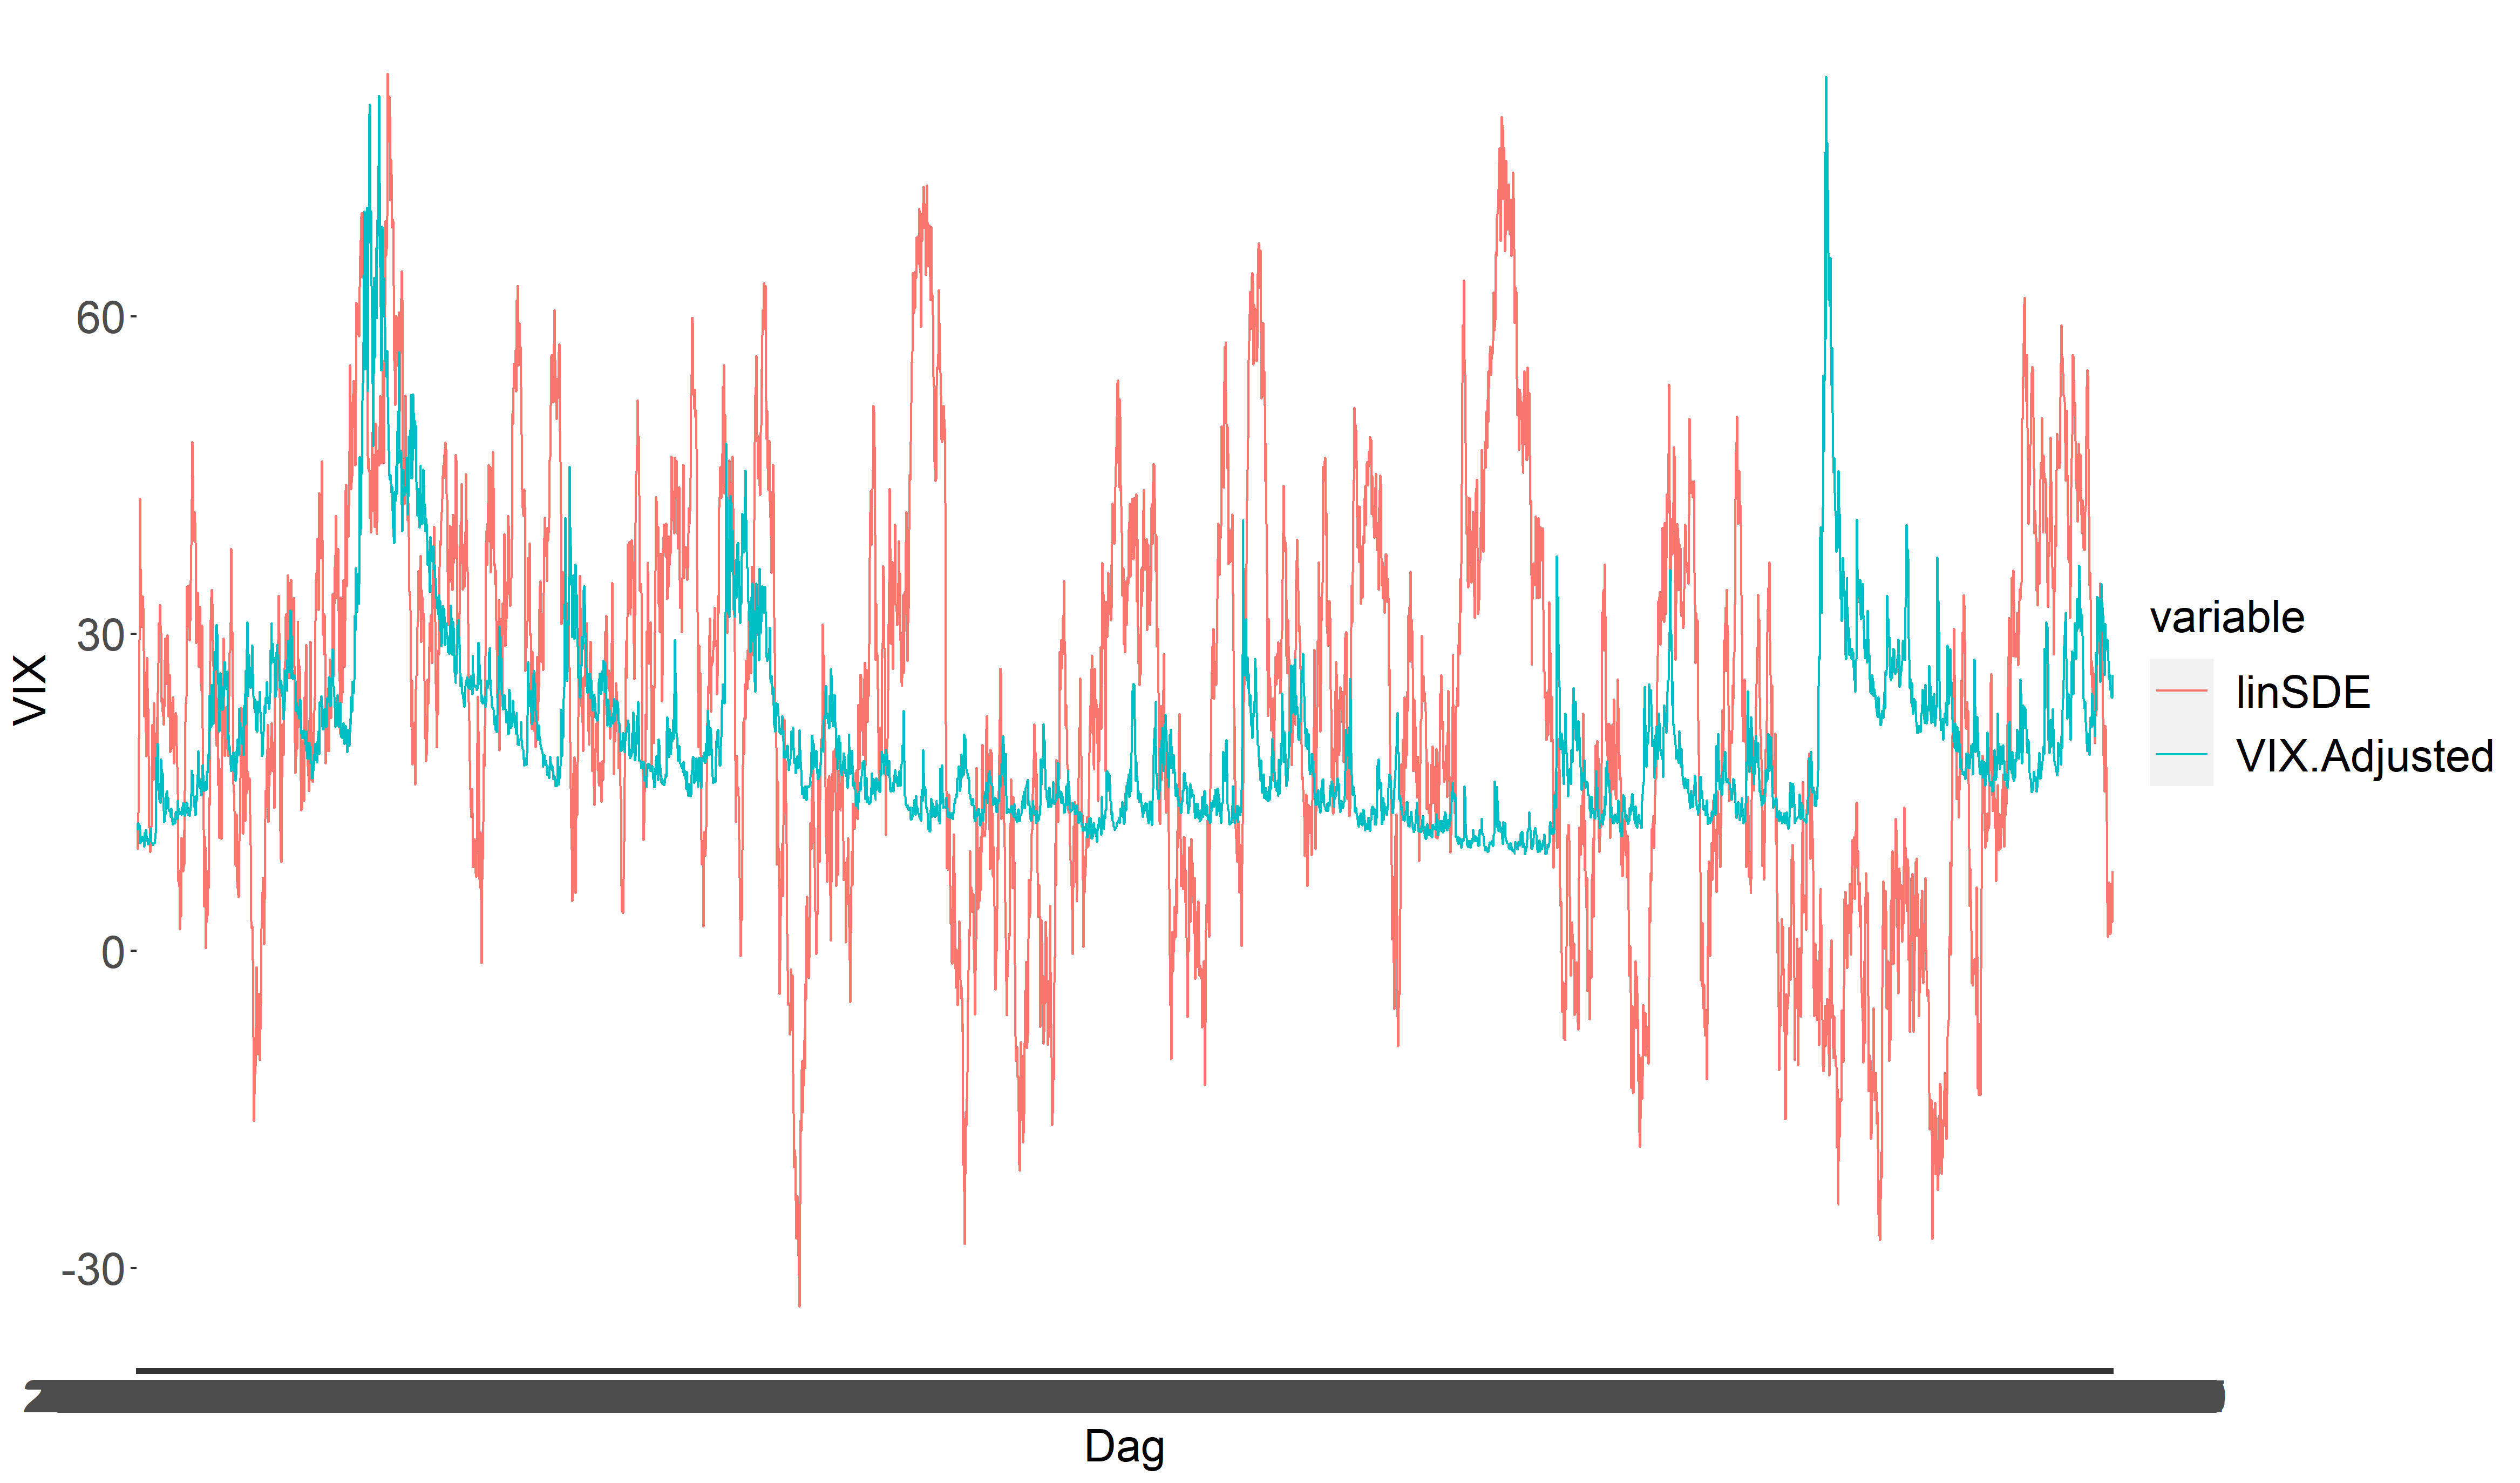
\includegraphics[width=2in]{simul_VIX_OU}
    \caption{VIX vs. SDE}
    \label{fig:VIX}
\end{subfigure}
\begin{subfigure}{2in}
    \raggedleft
    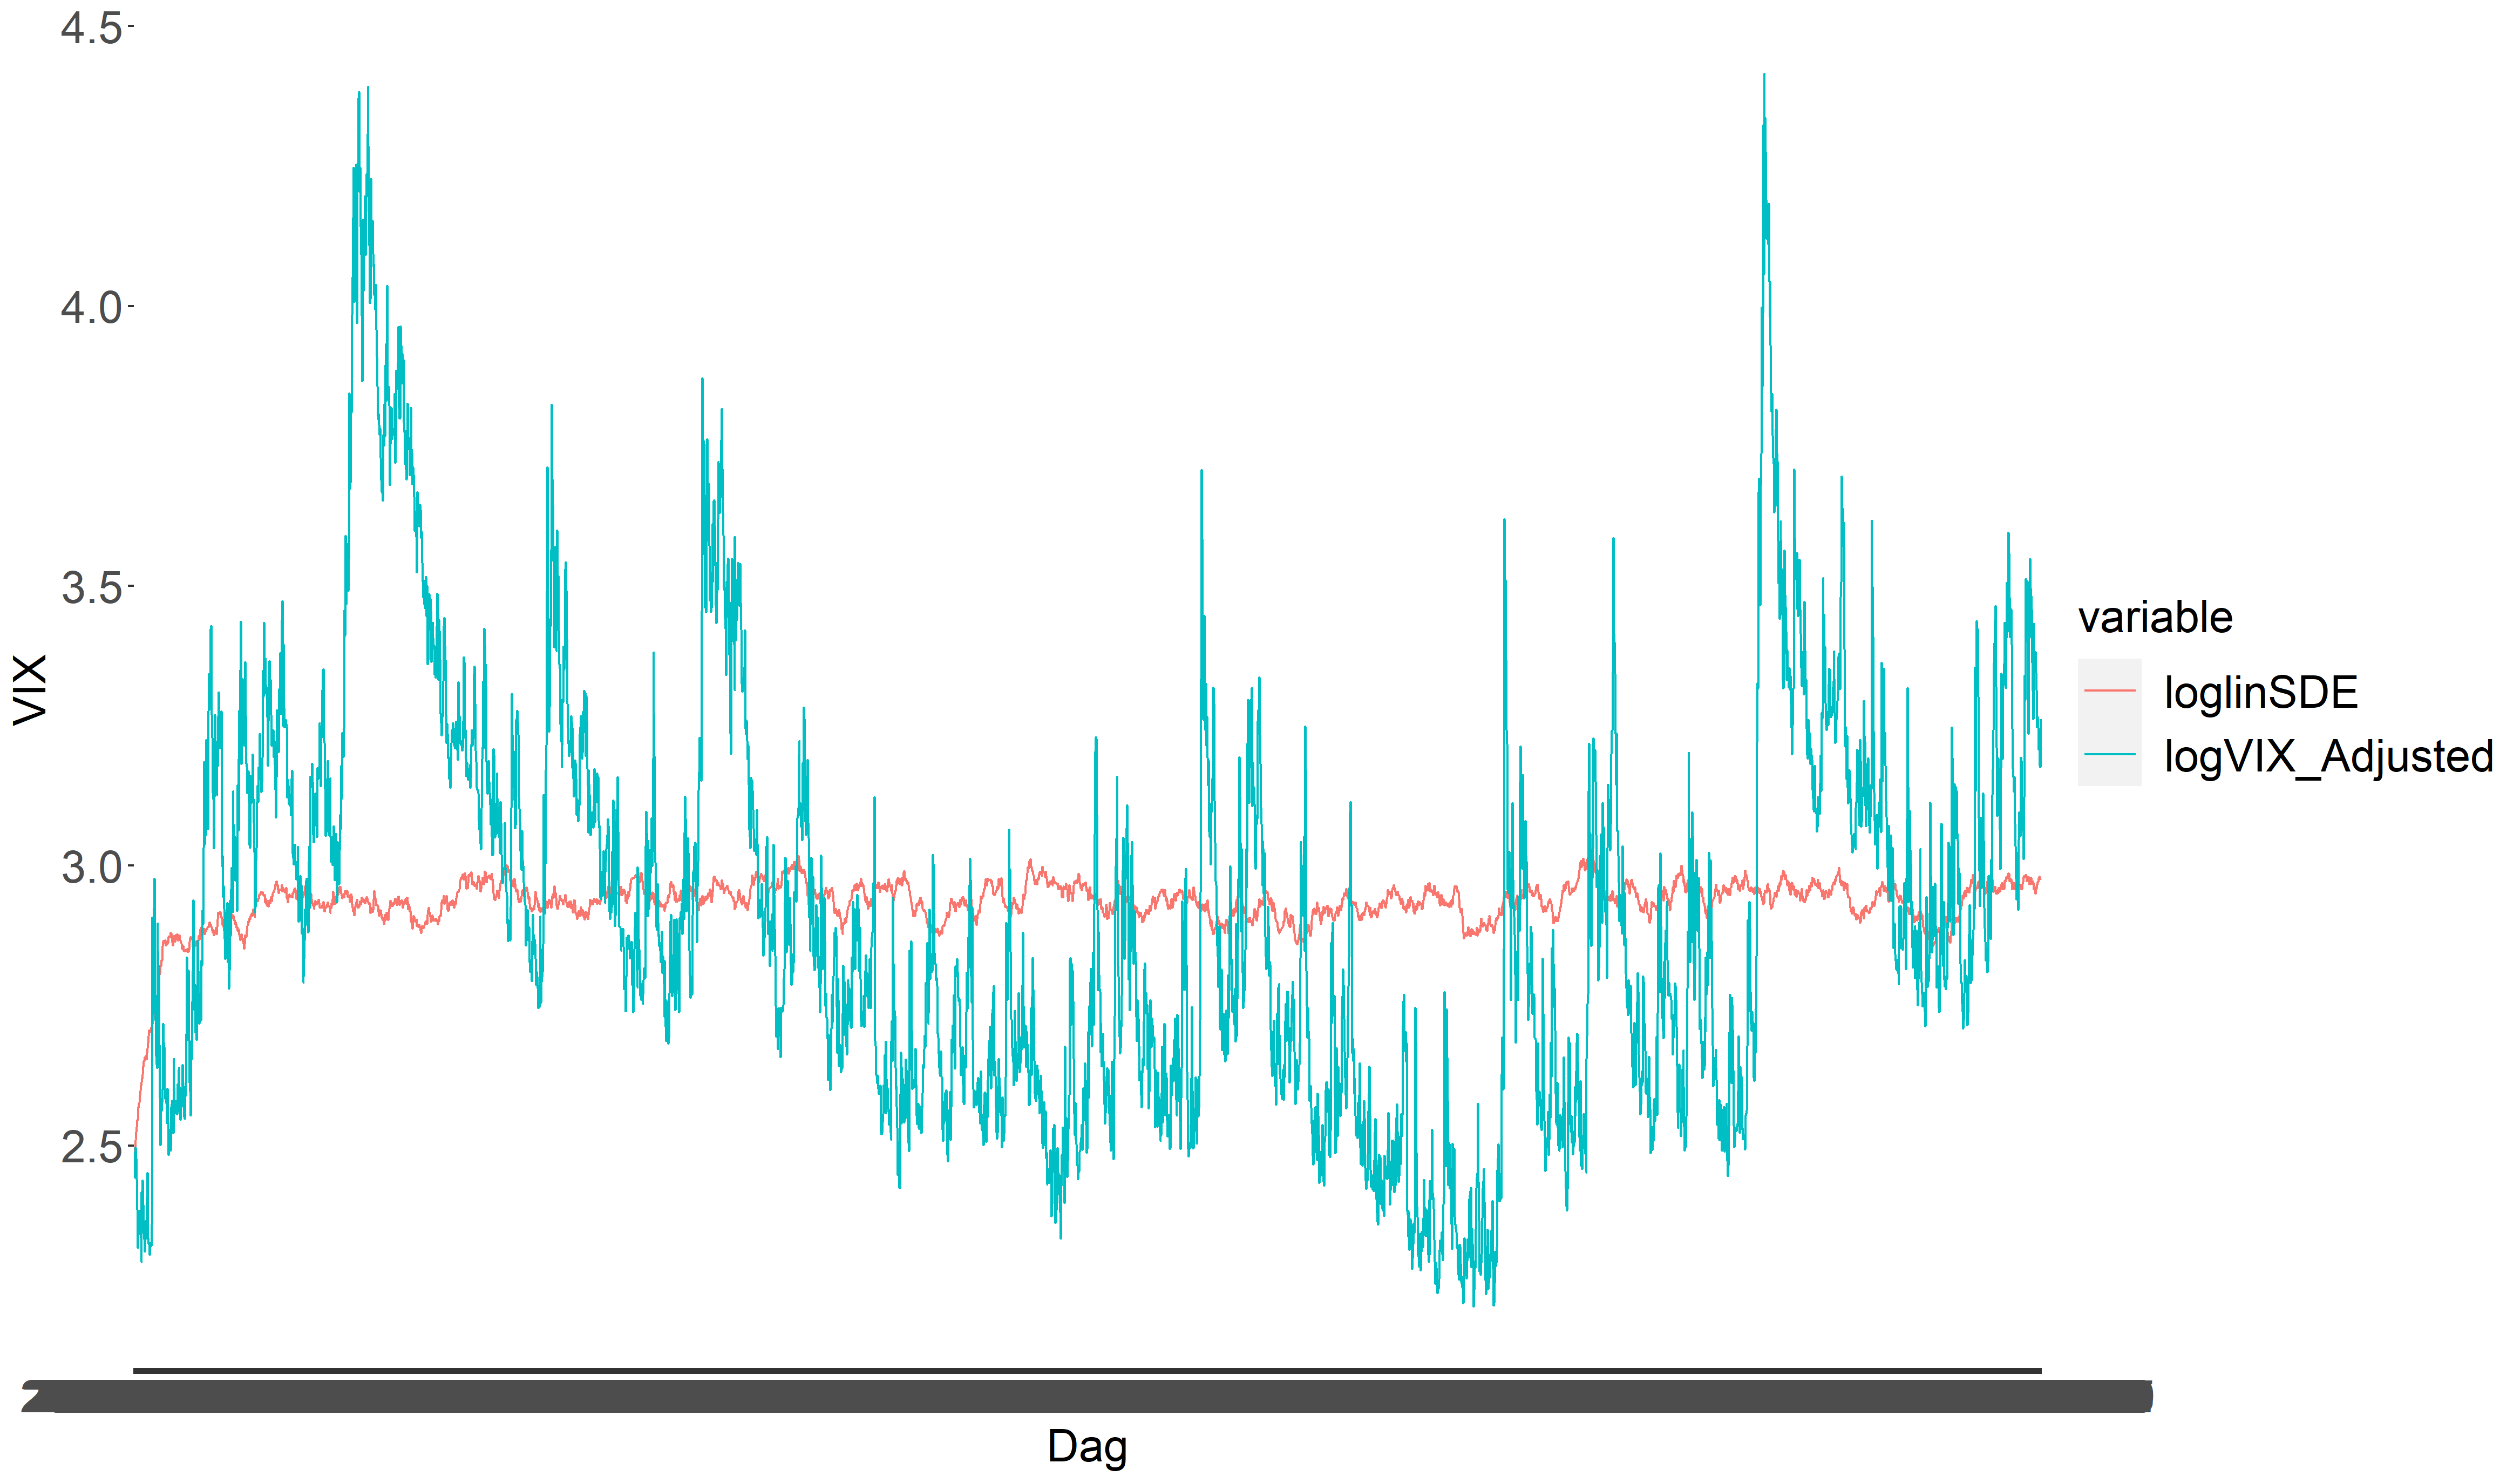
\includegraphics[width=2in]{simul_lnVIX_OU}
    \caption{lnVIX vs. SDE}
    \label{fig:logVIX}
\end{subfigure}
\end{figure}
Man ser her, at vores processer følger ln(VIX) bedre end VIX, selvom der stadig er tydelige afvigelser, idet processerne ikke ligner dataen. Vi kan også kigge på vores antagelse om at VIX er normalfordelt. Nedenfor ses 2 QQ-plot, der kan hjælpe med at bedømme, hvilken data-serie der passer bedst med normalfordelings antagelsen.
\begin{center}
    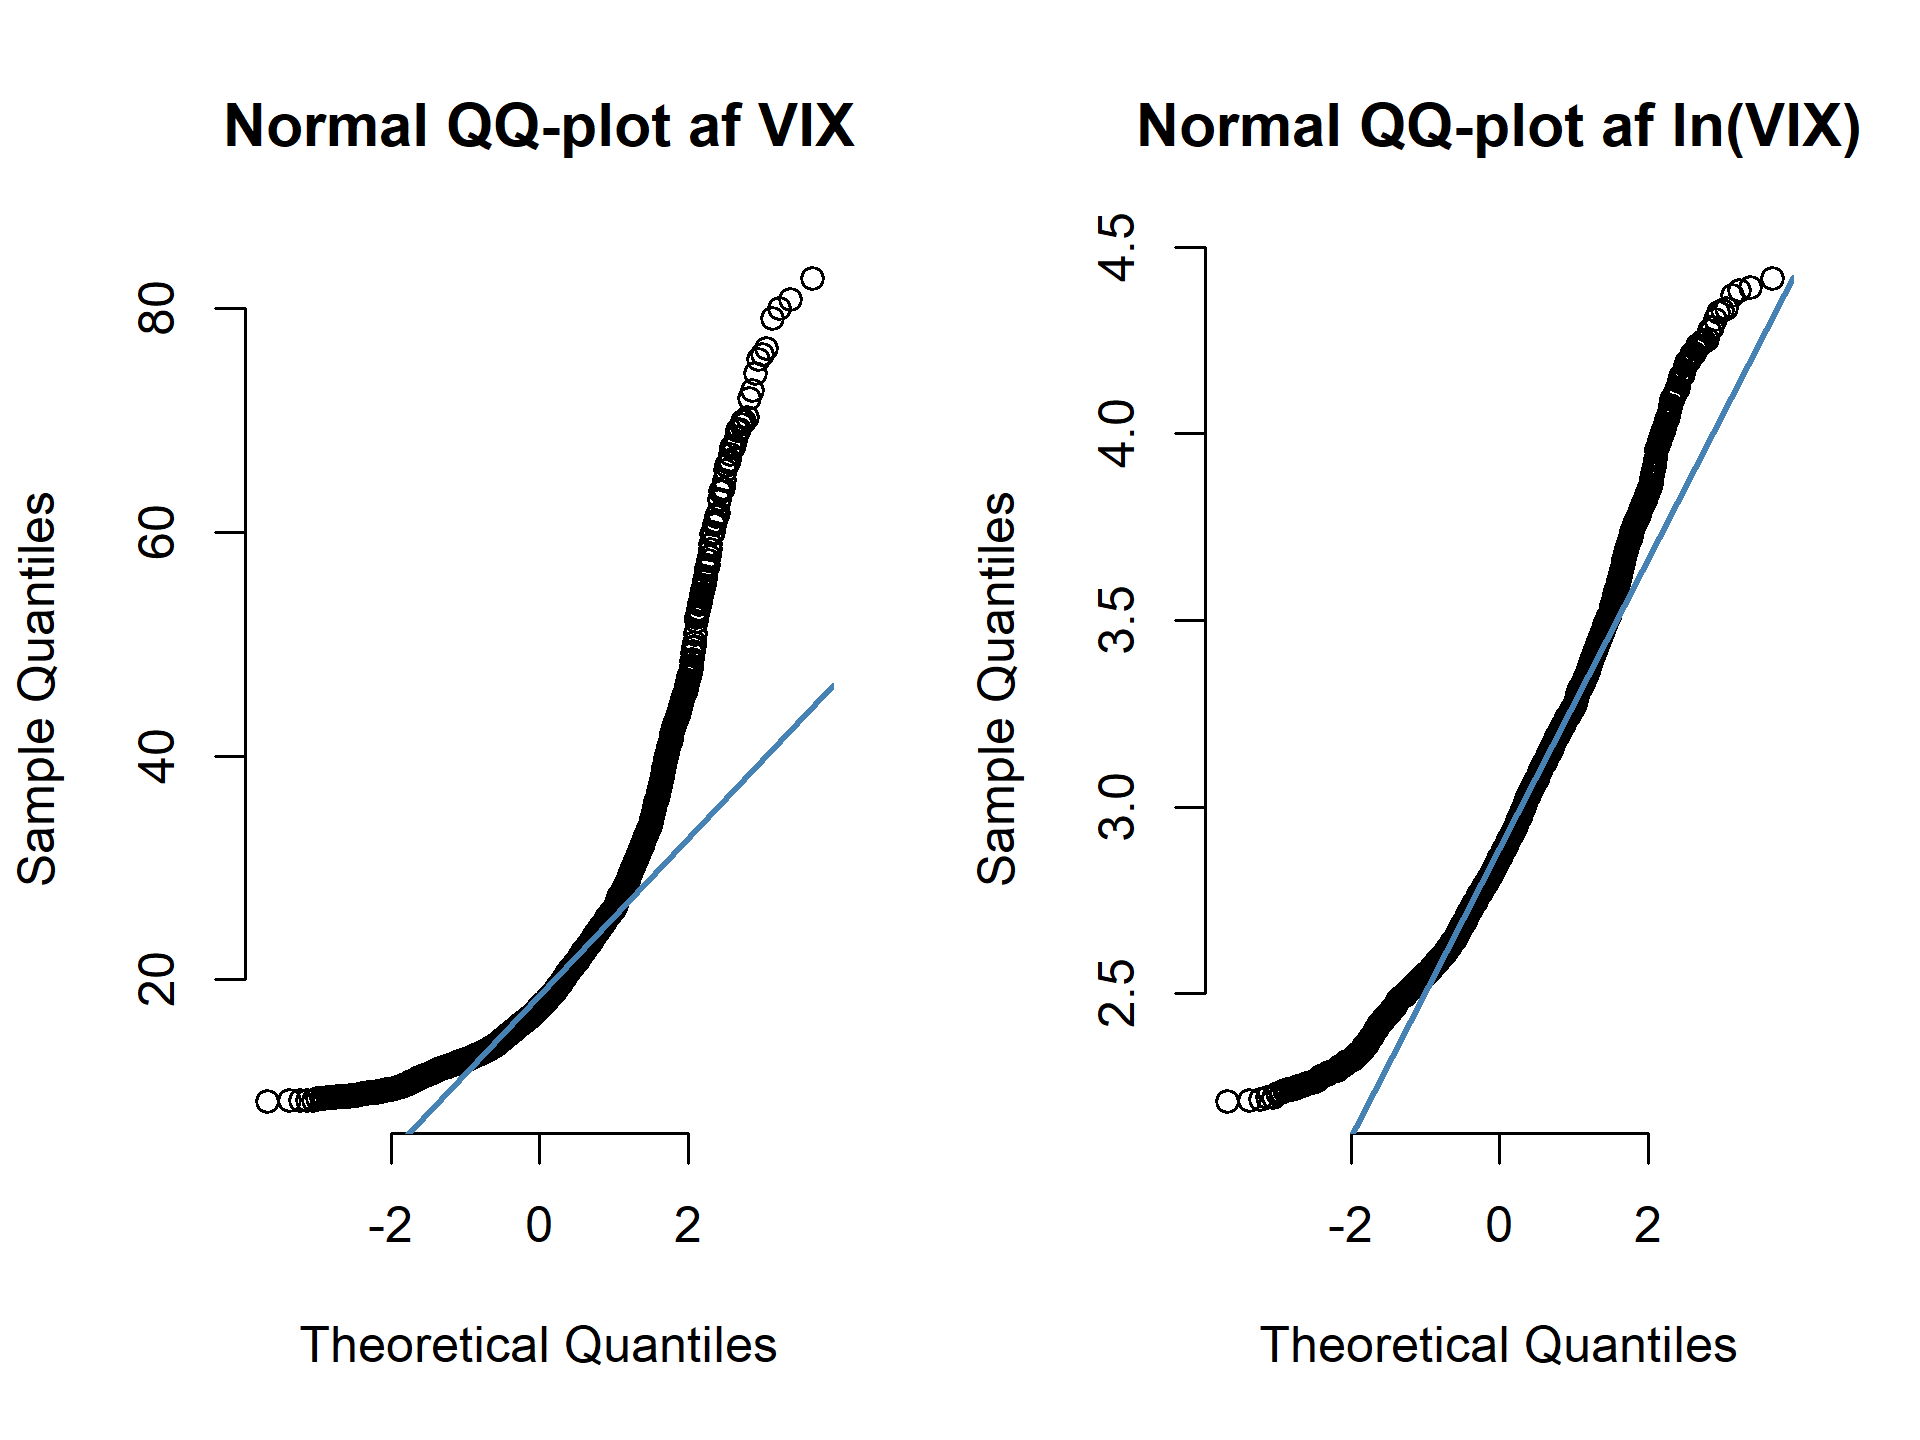
\includegraphics[width=4in]{QQ_VIX_vs_lnVIX}
\end{center}
Her ses det at ln(VIX) ligger mere normal fordelt i forhold til kvantilerne end VIX gør. Vi kan derfor konkludere, at ln(VIX)-modellen passer bedst til dataene.
\section{Pricing and hedging in the Black-Scholes model}
\subsection{Europæisk call option}
Til at starte med udledes et brugbart resultat. Vi definerer først en stokastisk differential ligning for en geometrisk brownsk bevægelse.
$$\text d X_t = \beta X_t\text dt+\xi X_t \text dW_t$$
Og funktionen samt procesen.
$$f(t,x)=e^{(\beta-\alpha)(T-t)}x,\quad Y_t=f(t,X_t)=e^{(\beta-\alpha)(T-t)}X_t$$
Vi kan nu finde $X_t$ ved brug af itô's formel, proposition 4.12 i Björk \cite{Bjork2020}.
$$\text dY_t=-(\beta-\alpha)e^{(\beta-\alpha)(T-t)}X_t\text d_t+e^{(\beta-\alpha)(T-t)}\text dX_t$$
$$=-(\beta-\alpha)e^{(\beta-\alpha)(T-t)}X_t\text dt+e^{(\beta-\alpha)(T-t)}(\beta X_t\text dt+\xi X_t\text dW_t)$$
$$=e^{(\beta-\alpha)(T-t)}X_t(\beta-(\beta-\alpha))\text dt+\xi X_t\text dW_t$$
$$=e^{(\beta-\alpha)(T-t)}X_t\alpha\text dt+\xi X_t\text dW_t$$
Vi bruger Björks proposition 7.13 \cite{Bjork2020}, hvor ligning (7.53) og (7.54) giver os at
$$d_1(t,Y_0) :=\frac{1}{\xi\sqrt{T-0}}\left[\ln\left(\frac{Y_0}{K}\right)+(\alpha+\frac12\xi)(T-0) \right]$$
$$=\frac{T(\beta-\alpha)+\ln\left(\frac{X_0}{K}\right)+(\alpha+\frac12\xi)T}{\xi\sqrt T}=\frac{\ln\left(\frac{X_0}{K}\right)+(\beta+\frac12\xi^2)T}{\xi\sqrt T}$$
$$d_2(t,Y_0):=\frac{\ln\left(\frac{X_0}{K}\right)+(\beta+\frac12\xi^2)T}{\xi\sqrt T}-\xi\sqrt{T}$$
$$=\frac{\ln\left(\frac{X_0}{K}\right)+(\beta+\frac12\xi^2)T-\xi^2T}{\xi\sqrt T}=\frac{\ln\left(\frac{X_0}{K}\right)+(\beta-\frac12\xi^2)T}{\xi\sqrt T}$$
Og dermed får vi det nyttige resultat, som kan ses som en tid T pris tilbage diskonteret til tid t for europæisk call option.
$$F(t,Y_0)=Y_0\Phi(d_1)-e^{-\alpha T}K\Phi(d_2)$$
$$=e^{(\beta-\alpha)T}X_0\Phi\left(\frac{\ln\left(\frac{X_0}{K}\right)+(\beta+\frac12\xi^2)T}{\xi\sqrt T}\right)-e^{-\alpha T}K\Phi\left(\frac{\ln\left(\frac{X_0}{K}\right)+(\beta-\frac12\xi^2)T}{\xi\sqrt T}\right)$$
Endvidere kunne vi tænke os at finde tid $t-\Delta$'et for vores europæiske call-option i markedet.
$$\text dB_t = rB_t\text d_t$$
$$\text d S_t = \mu S_t\text d_t +\sigma \text dW_t^P$$
P skal her forstås som aktie-pris dynamikken. Pris processen $B_t$ er her det risiko fri aktiv, og pris-processen $S_t$ er aktie kuren. $\mu,r$ og $\sigma>0$ er konstanter. Björks proposition 7.13 \cite{Bjork2020} fortæller os nu at tid-t prisen på den europæiske call option er.
$$\Pi_t=F(t,S_t)=S_t\Phi\left(\frac{\ln\left(\frac{S_t}{K}\right)+(r+\frac12\sigma^2)(T-t)}{\sigma\sqrt{T-t}}\right)-e^{-r(T-t)}\Phi\left(\frac{\ln\left(\frac{S_t}{K}\right)+(r-\frac12\sigma^2)(T-t)}{\sigma\sqrt{T-t}}\right)$$
$$:= S_t\Phi(d_1^a)-e^{-r(T-t)}\Phi(d_2^a)$$
tid t-$\Delta$'et er da
$$\Delta(S_t,t) = \frac{\partial \Pi_t}{\partial S_t}=\Phi(d_1^a)+S_t\frac{\phi(d_1^a)}{S_t\sigma\sqrt{T-t}}-e^{-r(T-t)}K\frac{\phi(d_2^a)}{S_t\sigma\sqrt{T-t}}$$
$$=\Phi(d_1^a)+\frac{S_t\phi(d_1^a)-e^{-r(T-t)}K\phi(d_2^a)}{S_t\sigma\sqrt{T-t}}=\Phi(d_1^a)+\frac{S_t\phi(d_1^a)-S_t\phi(d_1^a)}{S_t\sigma\sqrt{T-t}}=\Phi(d_1^a)$$
Her er det brugt at $\phi(d_2^a)=\phi(d_1^a)\frac{S_t}{K}e^{r(T-t)}$, og at standard normalfordelingens tæthedsfunktion er navngivet $\phi$. Nedenfor vises udledning af vores trick.
$$\phi(d_2^a)=\phi(d_1^a-\sigma\sqrt{T-t})=\frac{1}{\sqrt{2\pi}}e^{-\frac12\left[(d_1^a)^2+\sigma^2(T-t)-2d_1^a\sqrt{T-t}\right]}$$
$$=\phi(d_1^a)e^{-\frac12\left[\sigma^2(T-t)-2d_1^a\sqrt{T-t}\right]}=\phi(d_1^a)e^{-\frac12\left[\sigma^2(T-t)-2\frac{\ln\left(\frac{S_t}{K}\right)+(r+\frac12\sigma^2)(T-t)}{\sigma\sqrt{T-t}}\sqrt{T-t}\right]}=\phi(d_1^a)\frac{S_t}{K}e^{r(T-t)}$$
\subsection{Digital option}
Ligeledes vil vi nu finde prisen på en digital option. Til det bruges Björks ligning (7.50) \cite{Bjork2020}, Q står her for det risiko neutrale mål. Vi definerer også et $\\Z\sim\mathcal N((r-\frac12\sigma^2)(T-t),\sigma\sqrt{T-t})$ og ligeledes dens henholdvise tæthedsfunktion $\phi_Z$ og fordelingsfunktion $\Phi_Z$. Derudover er $\Pi_t$ den arbitragefri tid-t pris. 
$$E^Q_{t,S_t}\left[1_{S_T\leq K}\right]=\int_{-\infty}^{\infty}1_{S_te^{z}\leq K}\phi_Z(z)\text dz=\int_{-\infty}^{\ln\left(\frac K{S_t}\right)}\phi_Z(z)\text d z=\Phi_Z\left(\ln\left(\frac{K}{S_t}\right)\right)$$
$$\ens \Pi_t=F(t,S_t)=e^{-r(T-t)}\Phi_Z\left(\ln\left(\frac{K}{S_t}\right)\right)$$
Vi er ligeledes interesseret i den tid t $\Delta$, som findes nedenfor for vores digitale option.
$$\Delta(S_t,t)=\frac{\partial \Pi_t}{\partial S_t}=e^{-r(T-t)}\phi_Z\left(\ln\left(\frac{K}{S_t}\right)\right)\frac{1}{K/S_t}\left(-\frac{K}{S_t^2}\right)=-e^{-r(T-t)}\phi_Z\left(\ln\left(\frac{K}{S_t}\right)\right)\frac{1}{S_t}$$
Dette er brugbart da det beskriver, hvor meget der skal investeres i det risiko fyldte aktiv (og der med også det risikofrie aktiv), hvis optionen skal Delta-hedges i Black-Scholes modellen.
\subsection{Hedging af en europæisk call option}
Et R program skrevet af Rolf Poulsen (og redigeret af mig, Jonas Wolff) der hedger optioner kan findes på \href{https://github.com/JonasW01ff/Bachelor-Projekt/blob/main/Rolf_Hedge_kode.R}{github.com/JonasW01ff/Bachelor-Projekt/blob/main/Rolf\_Hedge\_kode.R}. Koden udregner blandt andet for en europæisk call option antal aktier i det underliggende aktiv og værdi investeret i bankbogen ved brug af Björks Theorem 8.5 \cite{Bjork2020} til at replikere call optionen, som blandt andet siger at.
$$h^S_t=\frac{\partial \Pi_t}{\partial S_t}$$
$$h^B_tB_t=\Pi_t-S_t\frac{\partial \Pi_t}{\partial S_t}$$
Hvor $h^S_t$ skal forstås som antal aktier i det underliggende aktiv $S_t$, og $h^B_t$ som antal aktier i det risikofri aktiv (Dvs. $h^B_tB_t$ er antal kr. i bankbogen til tid t). Ud fra det kan den replikerende porteføljes værdi udregnes som
$$V^h_t=h^S_tS_t+h^B_tB_t=\Pi_t$$
Disse værdier udregnes Nhedge antal gange inden for løbetiden, med ækvidistante mellem rum (hvor Nhedge er en konstant). Man kan nu gøre dette et antal gange (her kaldet Nrep), og derefter sammenligne den replikerende porteføljes værdi, og optionens værdi $V^{Call}_t=\max(S_t-K,0)$. Dette er f.eks. gjort i koden ved at tage gennemsnitet af de tilbagediskonterede afvigelser. 

Skulle man være i en situation, hvor det underliggende aktivs drift ikke er lig bankbogens rente, da burde det ikke gøre noget, da vi ikke bryder med nogle antagelser i Black-Scholes modellen. Vi ser derfor også at hedge fejlene forbliver uændrede når renten er 0.1 fra vores aktie kurs' drift. Som det kan ses i figur \ref{fig:my_label5}, på næste side.
\begin{figure}
    \centering
    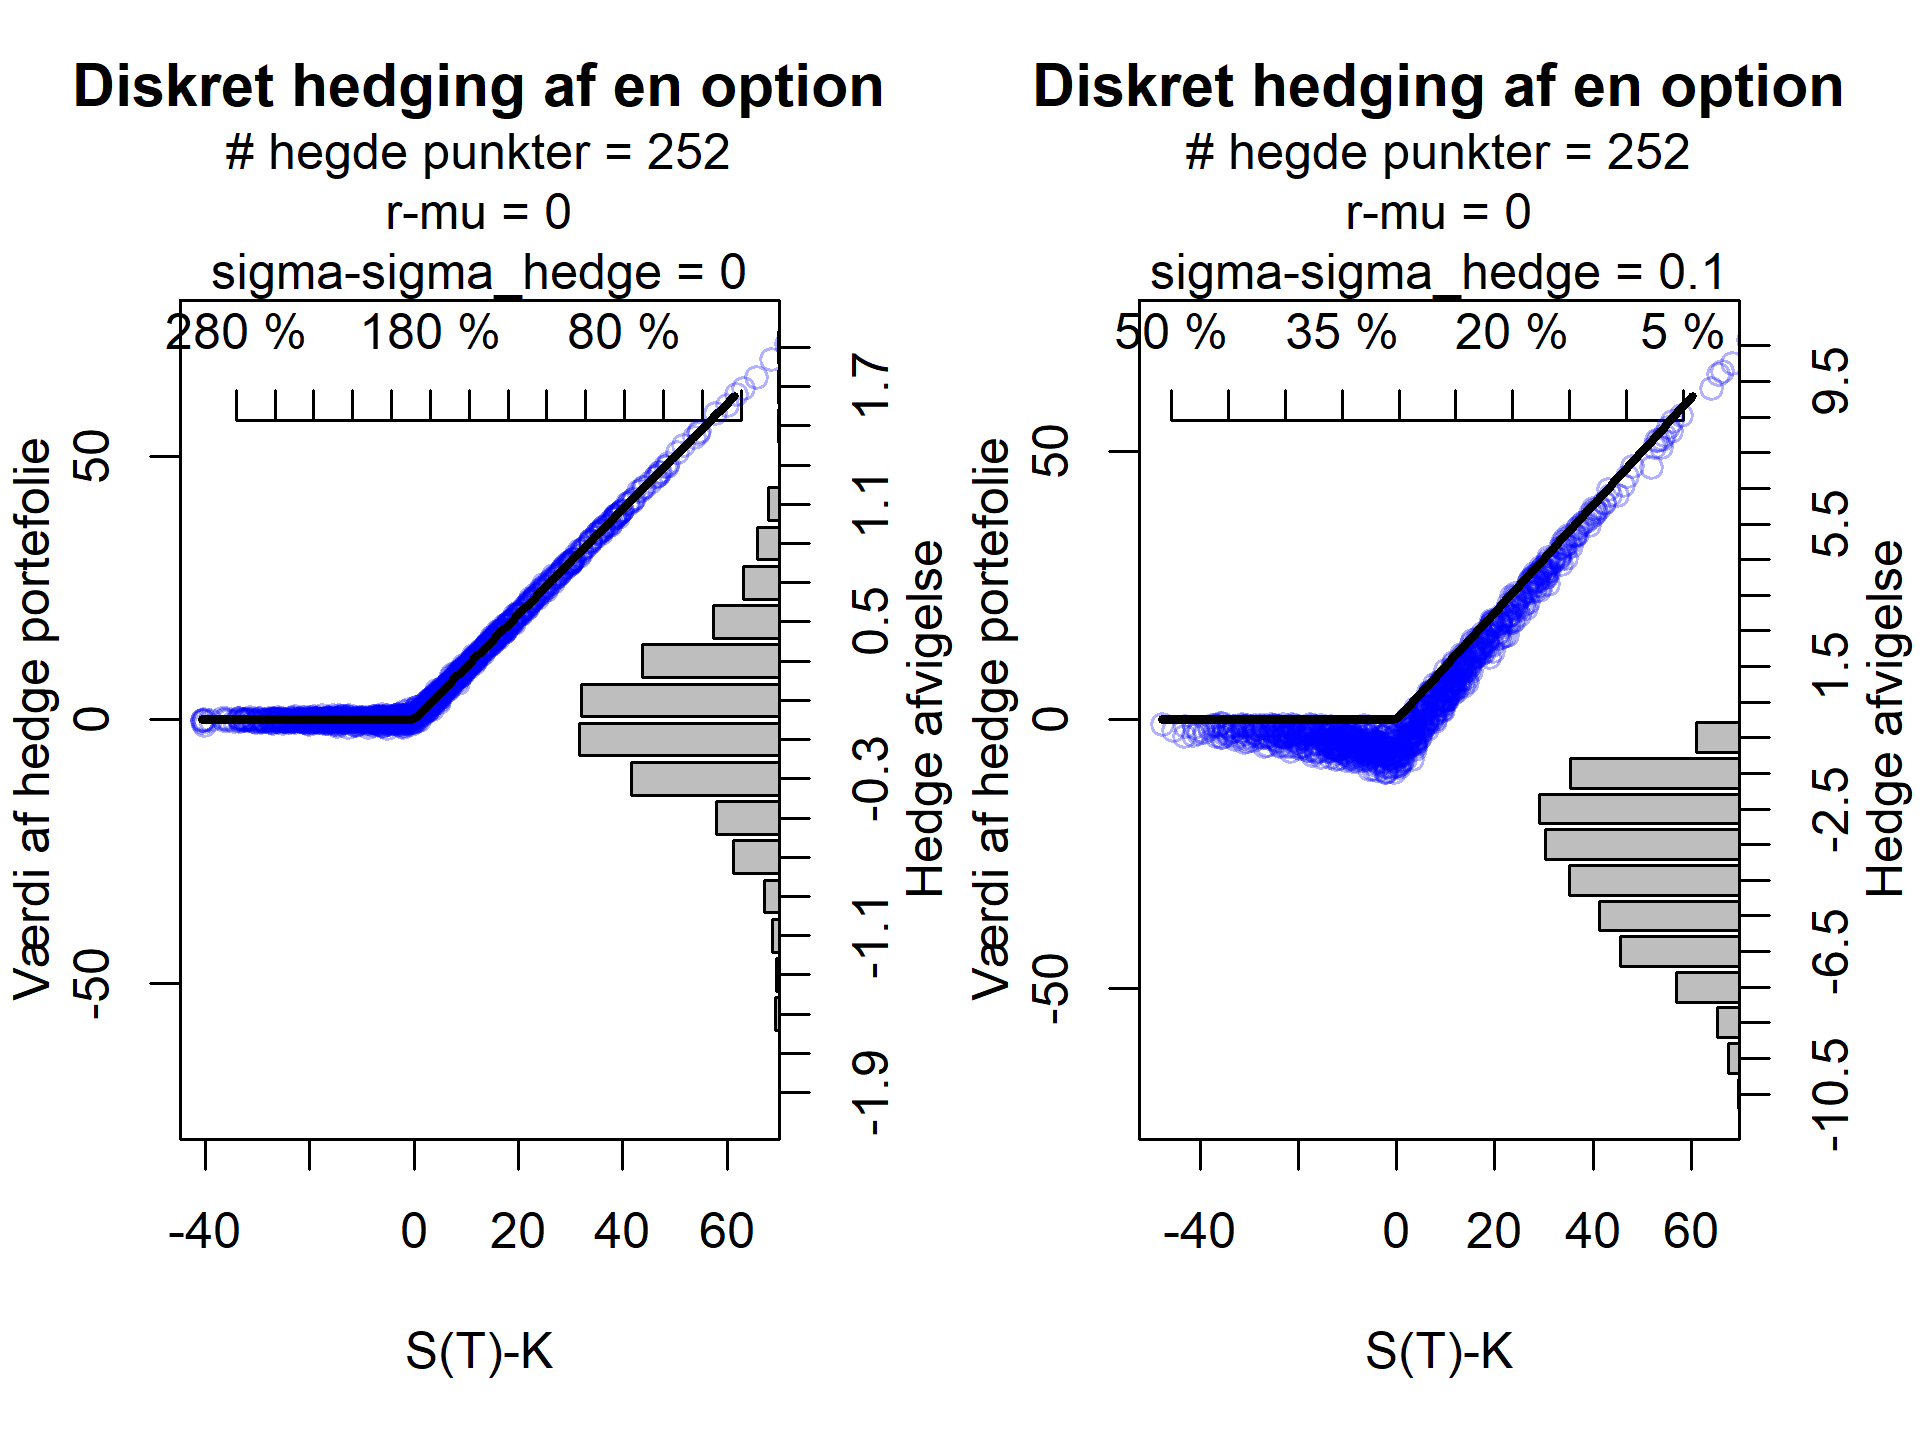
\includegraphics[width=3.5in]{Overleaf/1 opttype_standard_sigma.png}
    \caption{Endelig Hedge afvigelse i gns. hhv 0.331795943519772 og 3.92942369390872 Og Endelig Hedge afvigelses sd. hhv 0.443614523170148 og 2.00431398121781}
    \label{fig:my_label4}
\end{figure}

I tilfældet af at man ikke har fundet det rigtige $\sigma$ til at bruge i black-scholes, da ser vi tilgengæld at de endelige afvigelser mellem den replikerende portefølje og optionen øges. Dette er på grund af at teorien antager, at vi bruger volatiliteten der faktisk er på det risiko fyldte aktiv. Dette ses i figur \ref{fig:my_label4}
\begin{figure}
    \centering
    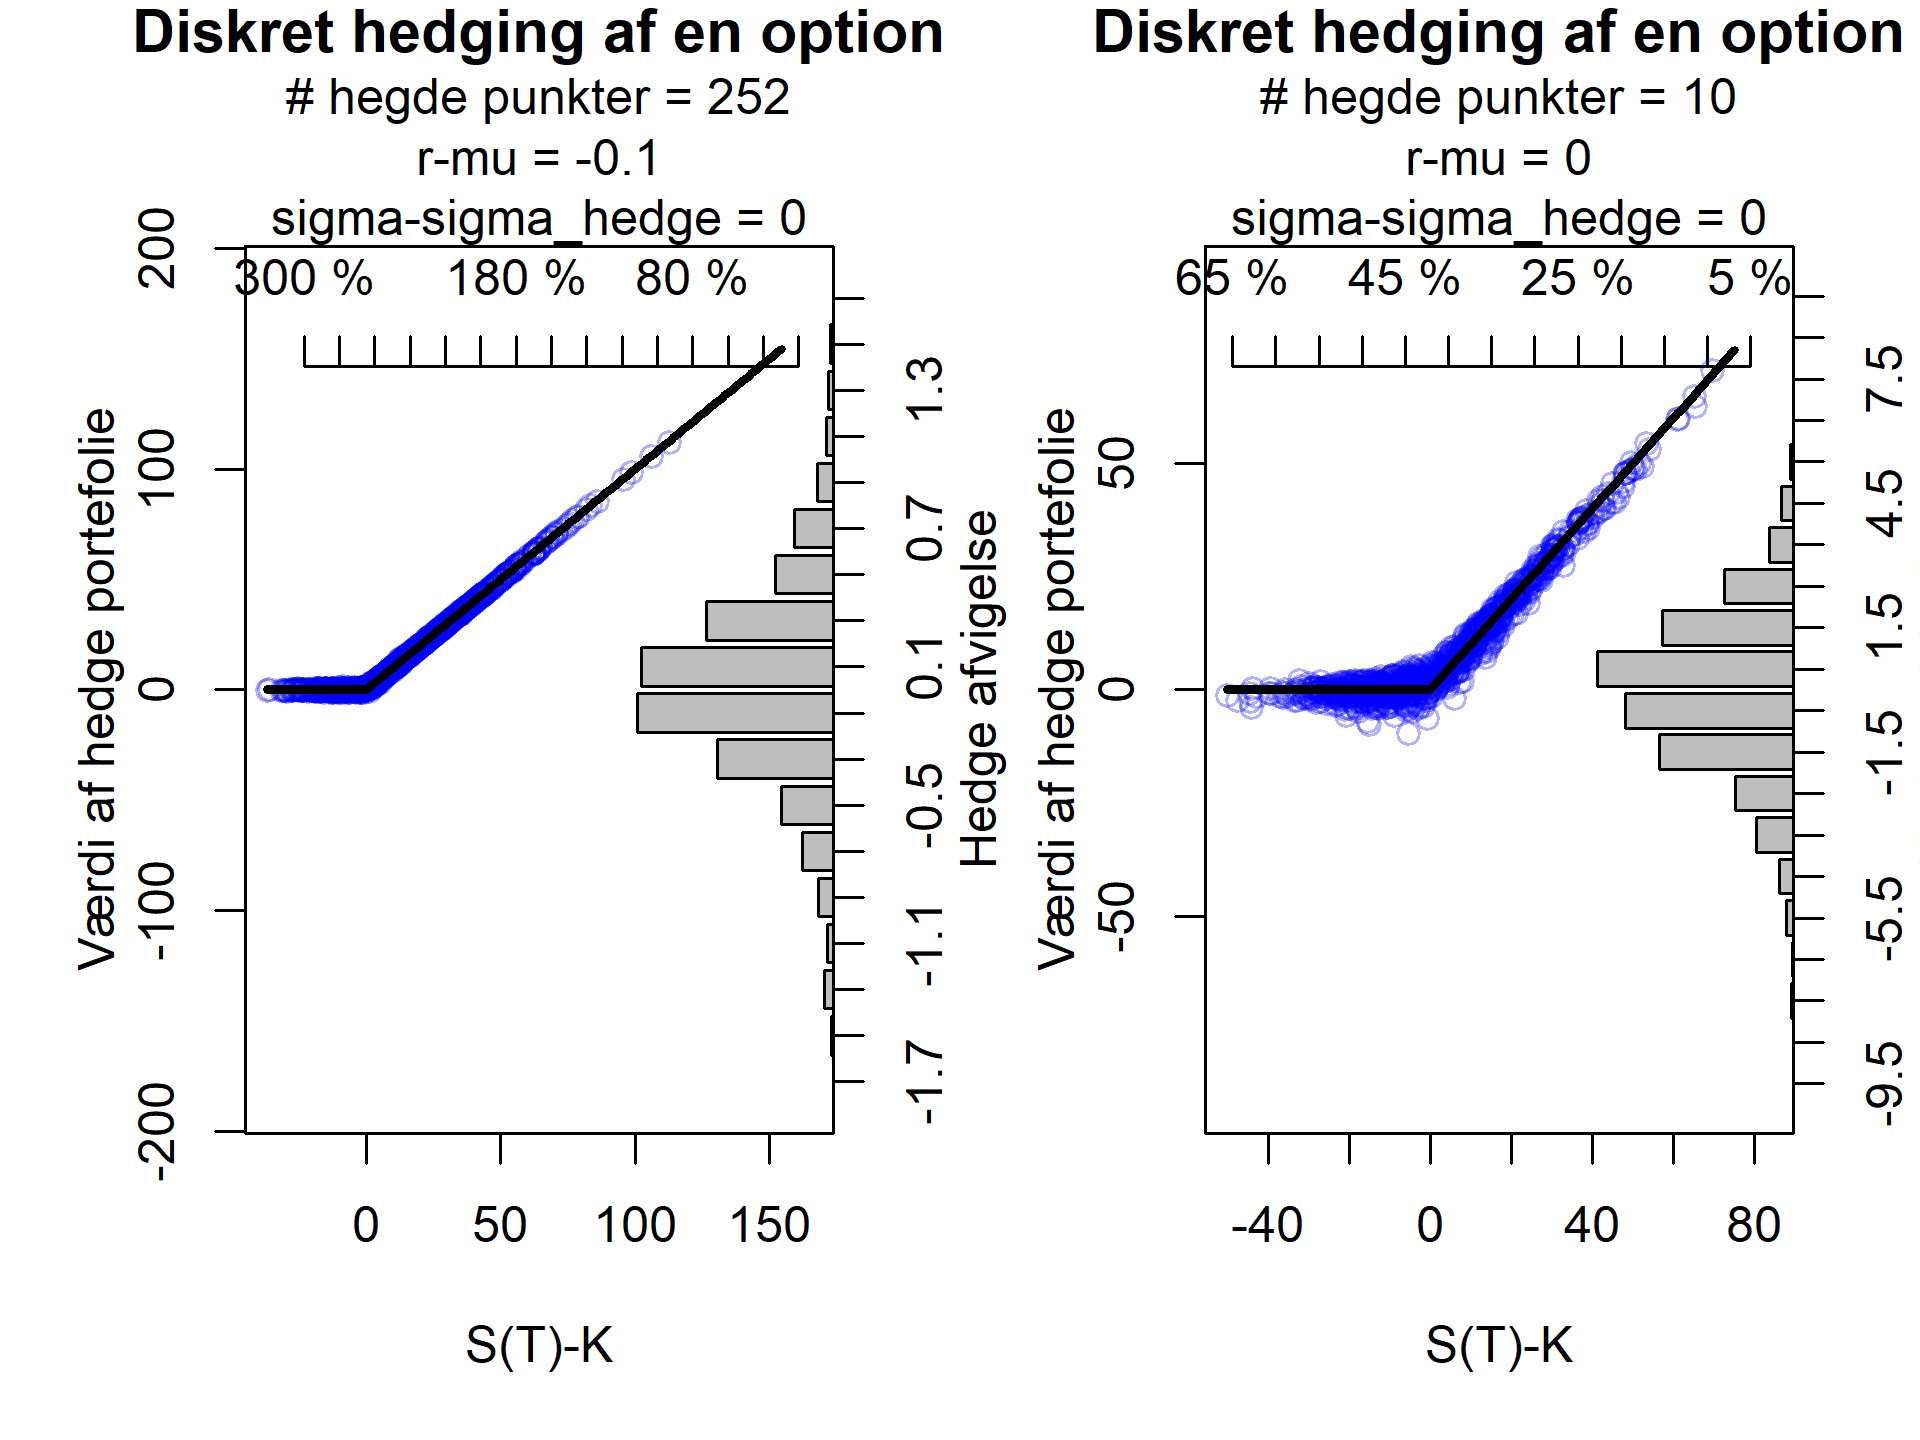
\includegraphics[width=3.5in]{Overleaf/1 opttype_mu_Nhedge.png}
    \caption{Endelig Hedge afvigelse i gns. hhv 0.325779051718594 og 1.65541985475094 Og Endelig Hedge afvigelses sd. hhv 0.4423721089574 og 2.18495945381076}
    \label{fig:my_label5}
\end{figure}

I forhold til at føre Björks Theorem 8.5 \cite{Bjork2020} ud i livet har vi også et problem i forhold til, at modellen antager, at vi rebalancerer kontinuert over løbetiden, hvilket som bekendt er umuligt. Derfor må vi approksimere ved at rebalancere så ofte som muligt; Det betyder at jo flere gange vi rebalancere, jo mere præcis bliver vores delta hedging. Standardafvigelsen på forskellen mellem den replikerende portefølje og option stiger derfor jo færre rebalanceringer vi laver (Det der i koden kaldes Nhedge). Det tilhørende resultat findes i figur \ref{fig:my_label5}.


Kigger vi derimod på den digitale option, ser vi, at præcisionen stadig ikke afhænger nævneværdigt af om driften er lig renten, selvom vi stadig gøre brug af Q-målet. På den anden side bliver vi meget afhængige af om vores estimerede sigma\_hedge faktisk er det rigtige sigma, da et forkert sigma\_hedge vil øge forskellen mellem den replikerende portefølje og optionen gevaldigt. Antalet at rebalanceringer Nhedge, har også en ret stor betydning da vores options payoff ikke er kontinuert, og vi derfor har brug for rebalanceringer ret tæt omkring striken, og da vores rebalancering i vores teori skal være ækvidistante, kan vi ikke gøre andet end at øge antallet af rebalanceringer. Nedenfor vises simulationerne. Resultatet ses i figure \ref{fig:my_label3} og \ref{fig:my_label2}.
\begin{figure}
    \centering
    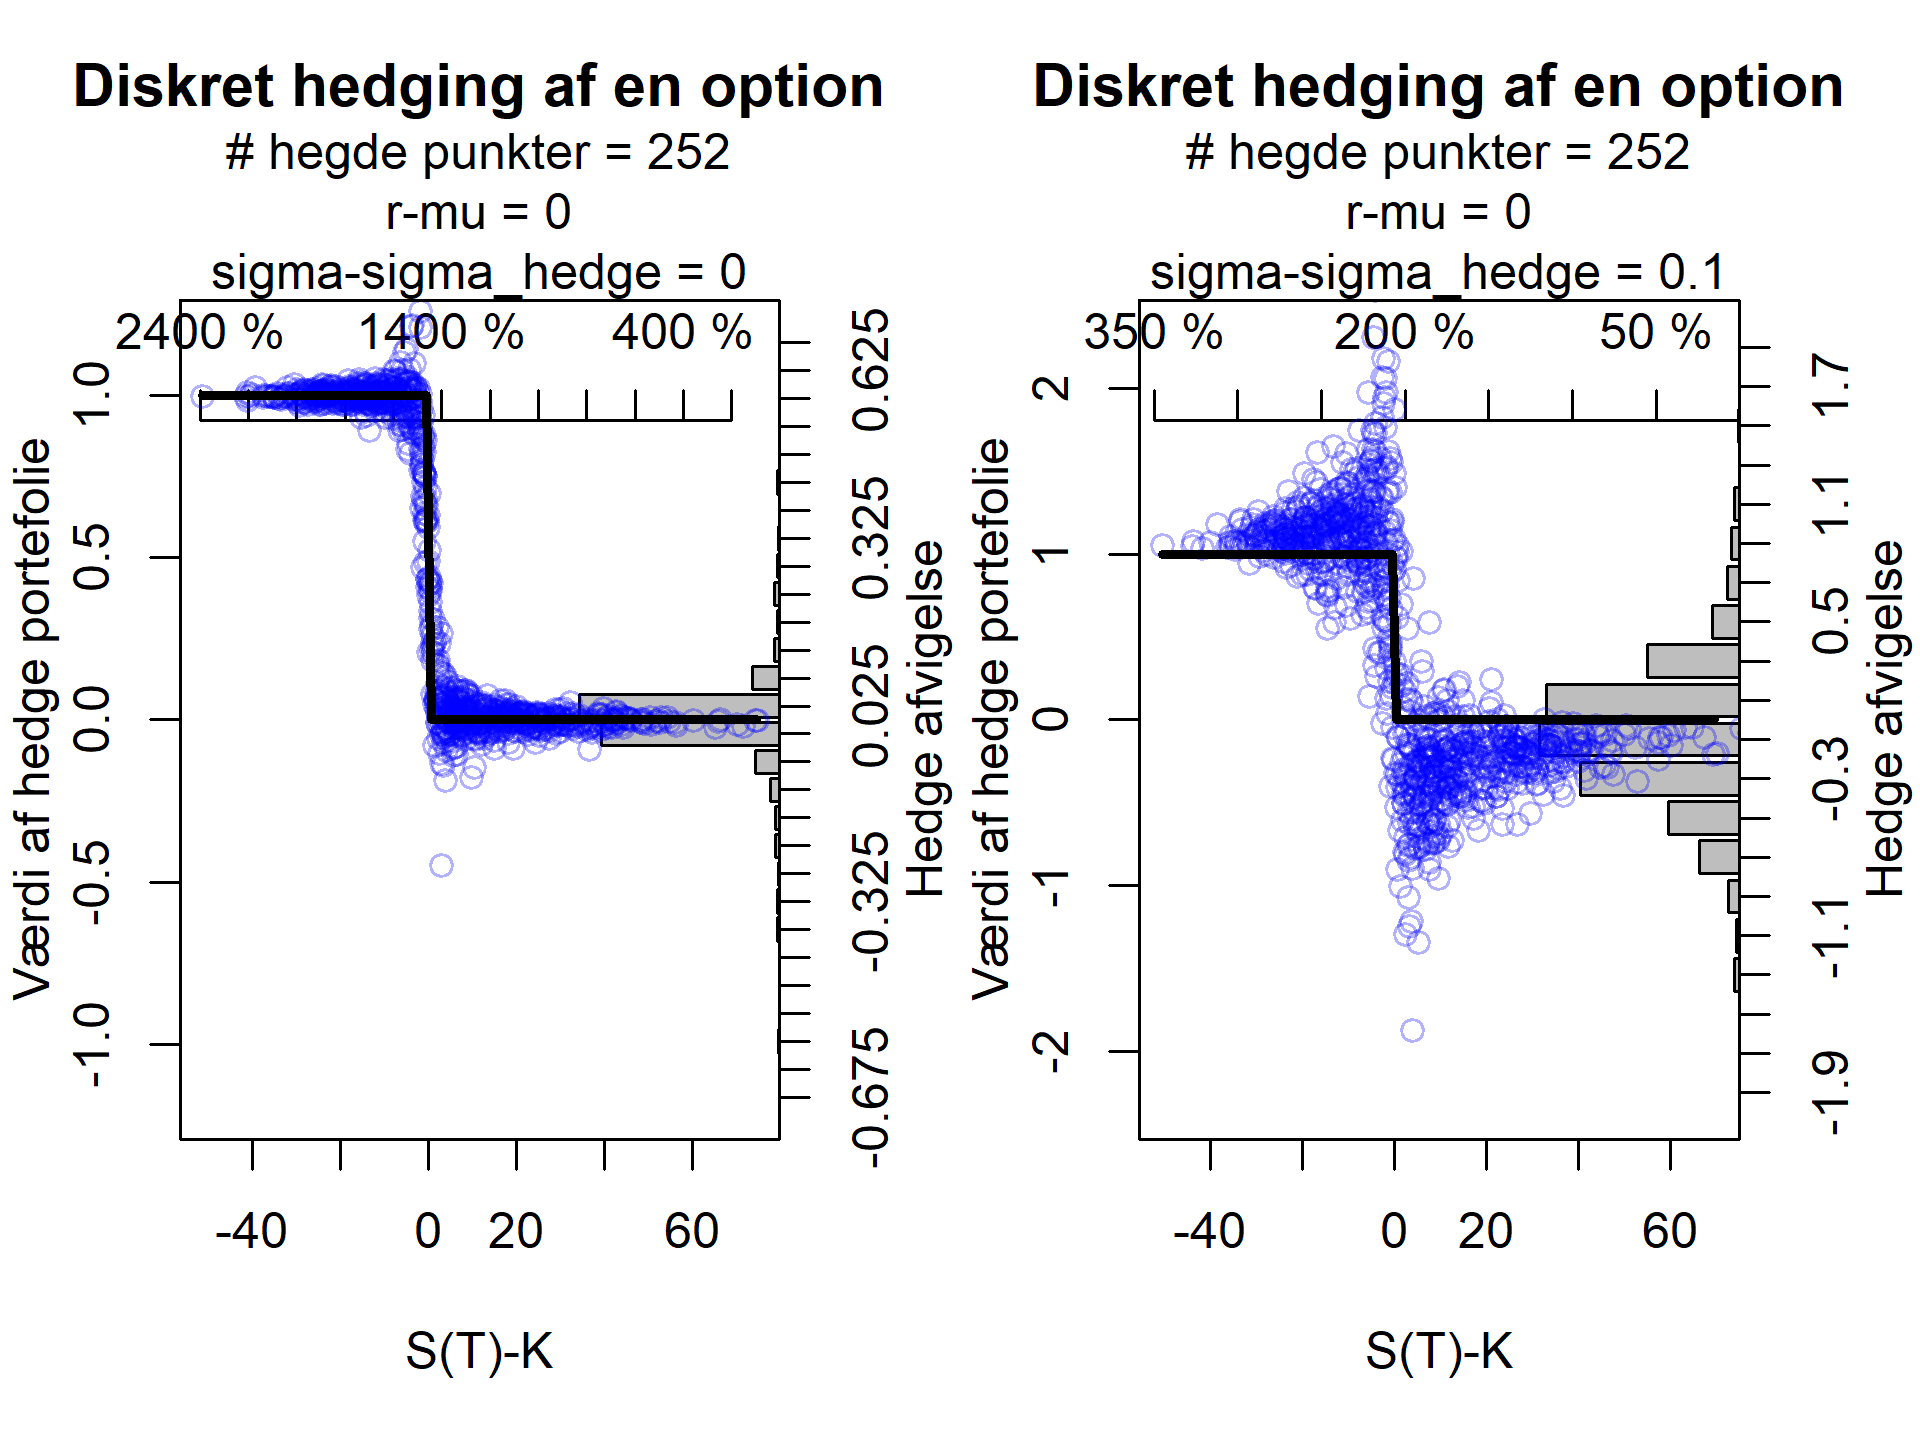
\includegraphics[width=3.5in]{Overleaf/3 opttype_standard_sigma.png}
    \caption{Endelig Hedge afvigelse i gns. hhv 0.0494206157323095 og 0.285544460843468 Og Endelig Hedge afvigelses sd. hhv 0.104386532078796 og 0.378316162933272}
    \label{fig:my_label3}
\end{figure}
\begin{figure}
    \centering
    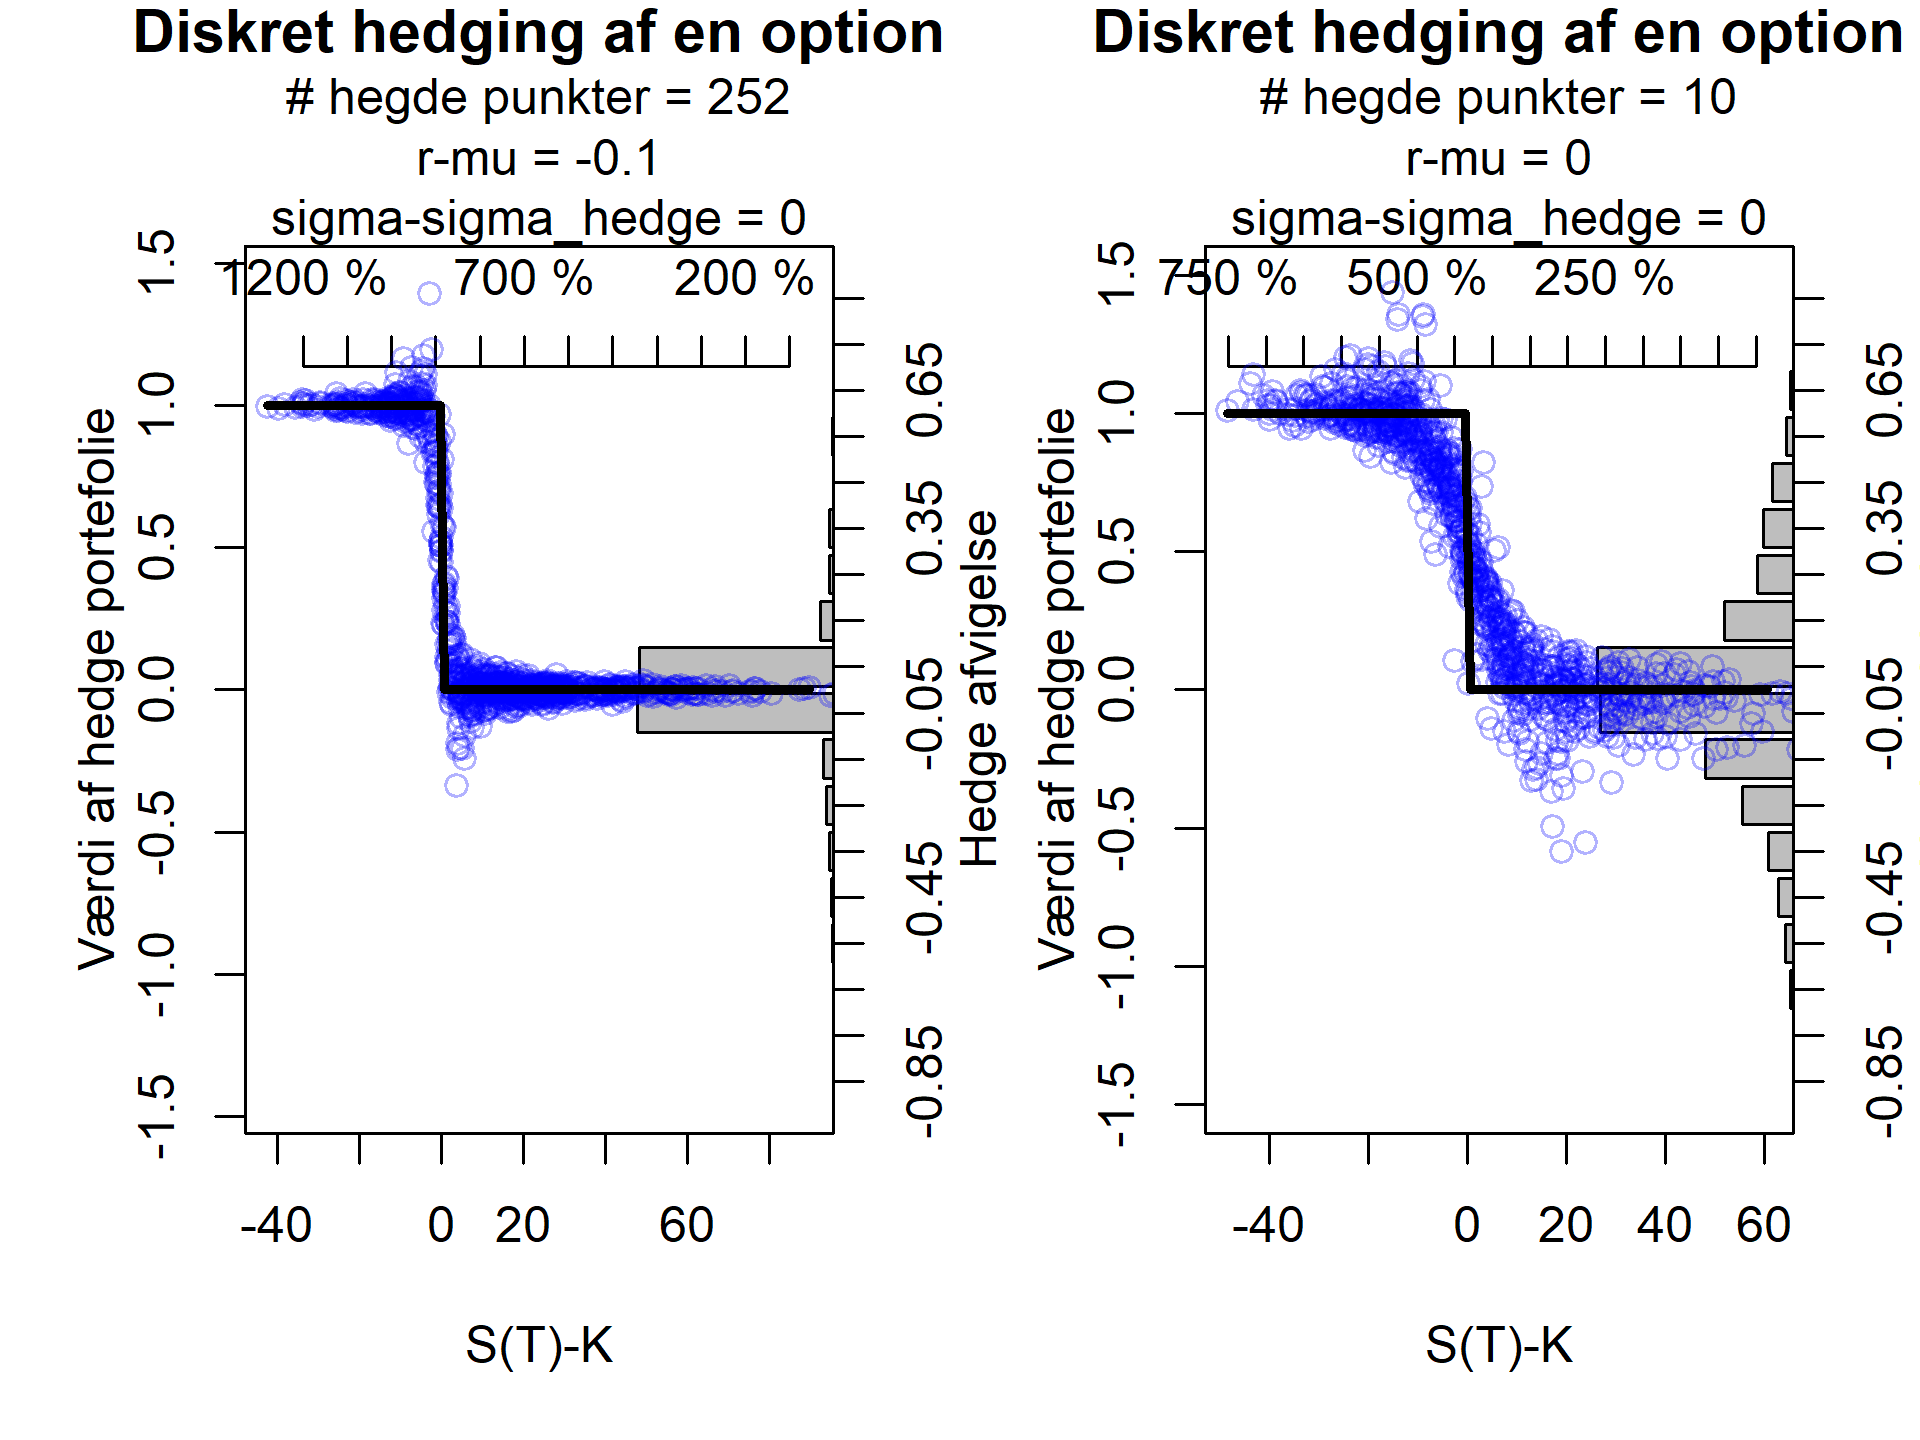
\includegraphics[width=3.5in]{Overleaf/3 opttype_mu_Nhedge.png}
    \caption{Endelig Hedge afvigelse i gns. hhv 0.0409730675718351 og 0.147414082399247 Og Endelig Hedge afvigelses sd. hhv 0.092565995966287 og 0.212102608359371}
    \label{fig:my_label2}
\end{figure}




\subsection{No touch digital option}
Præcis samme argumentation som i den almindelige digital option kan bruges her igen ved at bruge Björks ligning (7.50) \cite{Bjork2020}, hvor vi definere $M_t:=\max_{0\leq u\leq t}S_u$ som værende payoff for vores no touch digitale option
$$E^Q_{t,M_t}\left[1_{M_T\leq K}\right]=\int_{-\infty}^{\infty}1_{\max_{0\leq u\leq t} (S_ue^{z})\leq K}\phi_Z(z)\text dz=\int_{-\infty}^{\infty}1_{e^{z}M_t\leq K}\phi_Z(z)\text dz$$
$$=\int_{-\infty}^{\ln\left(\frac K{M_t}\right)}\phi_Z(z)\text d z=\Phi_Z\left(\ln\left(\frac{K}{S_t}\right)\right)\ens \Pi_t=F(t,S_t)=e^{-r(T-t)}\Phi_Z\left(\ln\left(\frac{K}{M_t}\right)\right)$$

\section{Empirisk hedging}
\subsection{Geometrisk Brownsk Bevægelse}
Vi starter med den stokastiske differential ligning nedenfor.
$$\text d X_t =  \mu X_t\text dt+\sigma X_t \text dW_t$$
Her indser vi at forventningen til vores støj led $\sigma S_t\text d W_t$ er 0. Vi kan nu omskrive vores stokastiske differential ligning til.
$$\frac{\text d X_t}{\text dt} =  \mu X_t+\sigma X_t \frac{\text dW_t}{\text dt}$$
Hvor vi nu tager forventningen på begge sider
$$\text E\left[\frac{\text d X_t}{\text dt}\right] =  \mu X_t$$
Vi indser hurtigt at $\text De^{\mu x}=\mu e^{\mu x}$. Vi får derfor at:
$$\text E[X_t|\mathcal F_u]=X_ue^{\mu (t-u)}$$
Vi har dermed løst den stokastiske differential ligning for $X_t$, da vi ved at $X_t$ er normal fordelt, eftersom det eneste stokastiske led i ligningen er $\text d W_t$ skaleret med konstant, hvilket jo er en skaleret normalfordeling, og dermed stadig en normal fordeling. Så vi har
$$X_t = X_{t-\Delta t}e^{\mu \Delta t}+\epsilon X_{t-\Delta t}\quad,\epsilon\sim\mathcal N(0,\sigma_\epsilon^2)$$
Eller
$$\text E[ln(X_t)|\mathcal F_{t-\Delta t}]=\text E[ln(X_{t-\Delta t})+\mu \Delta t]=ln(X_{t-\Delta t})+\mu \Delta t $$
Hvilket løses med almindelig lineær regression, hvor standard afvigelserne af residualerne divideret med $X_t$ giver os $\sigma_\epsilon$.
\subsection{S\&P500}
Vi vil nu udvide vore experiment til S\&P500, som ses på figur \ref{fig:VIXSP500}, hvor den første dato på både VIX og S\&P500 er normeret til 100, så de kan sammenlignes.
\begin{figure}
    \centering
    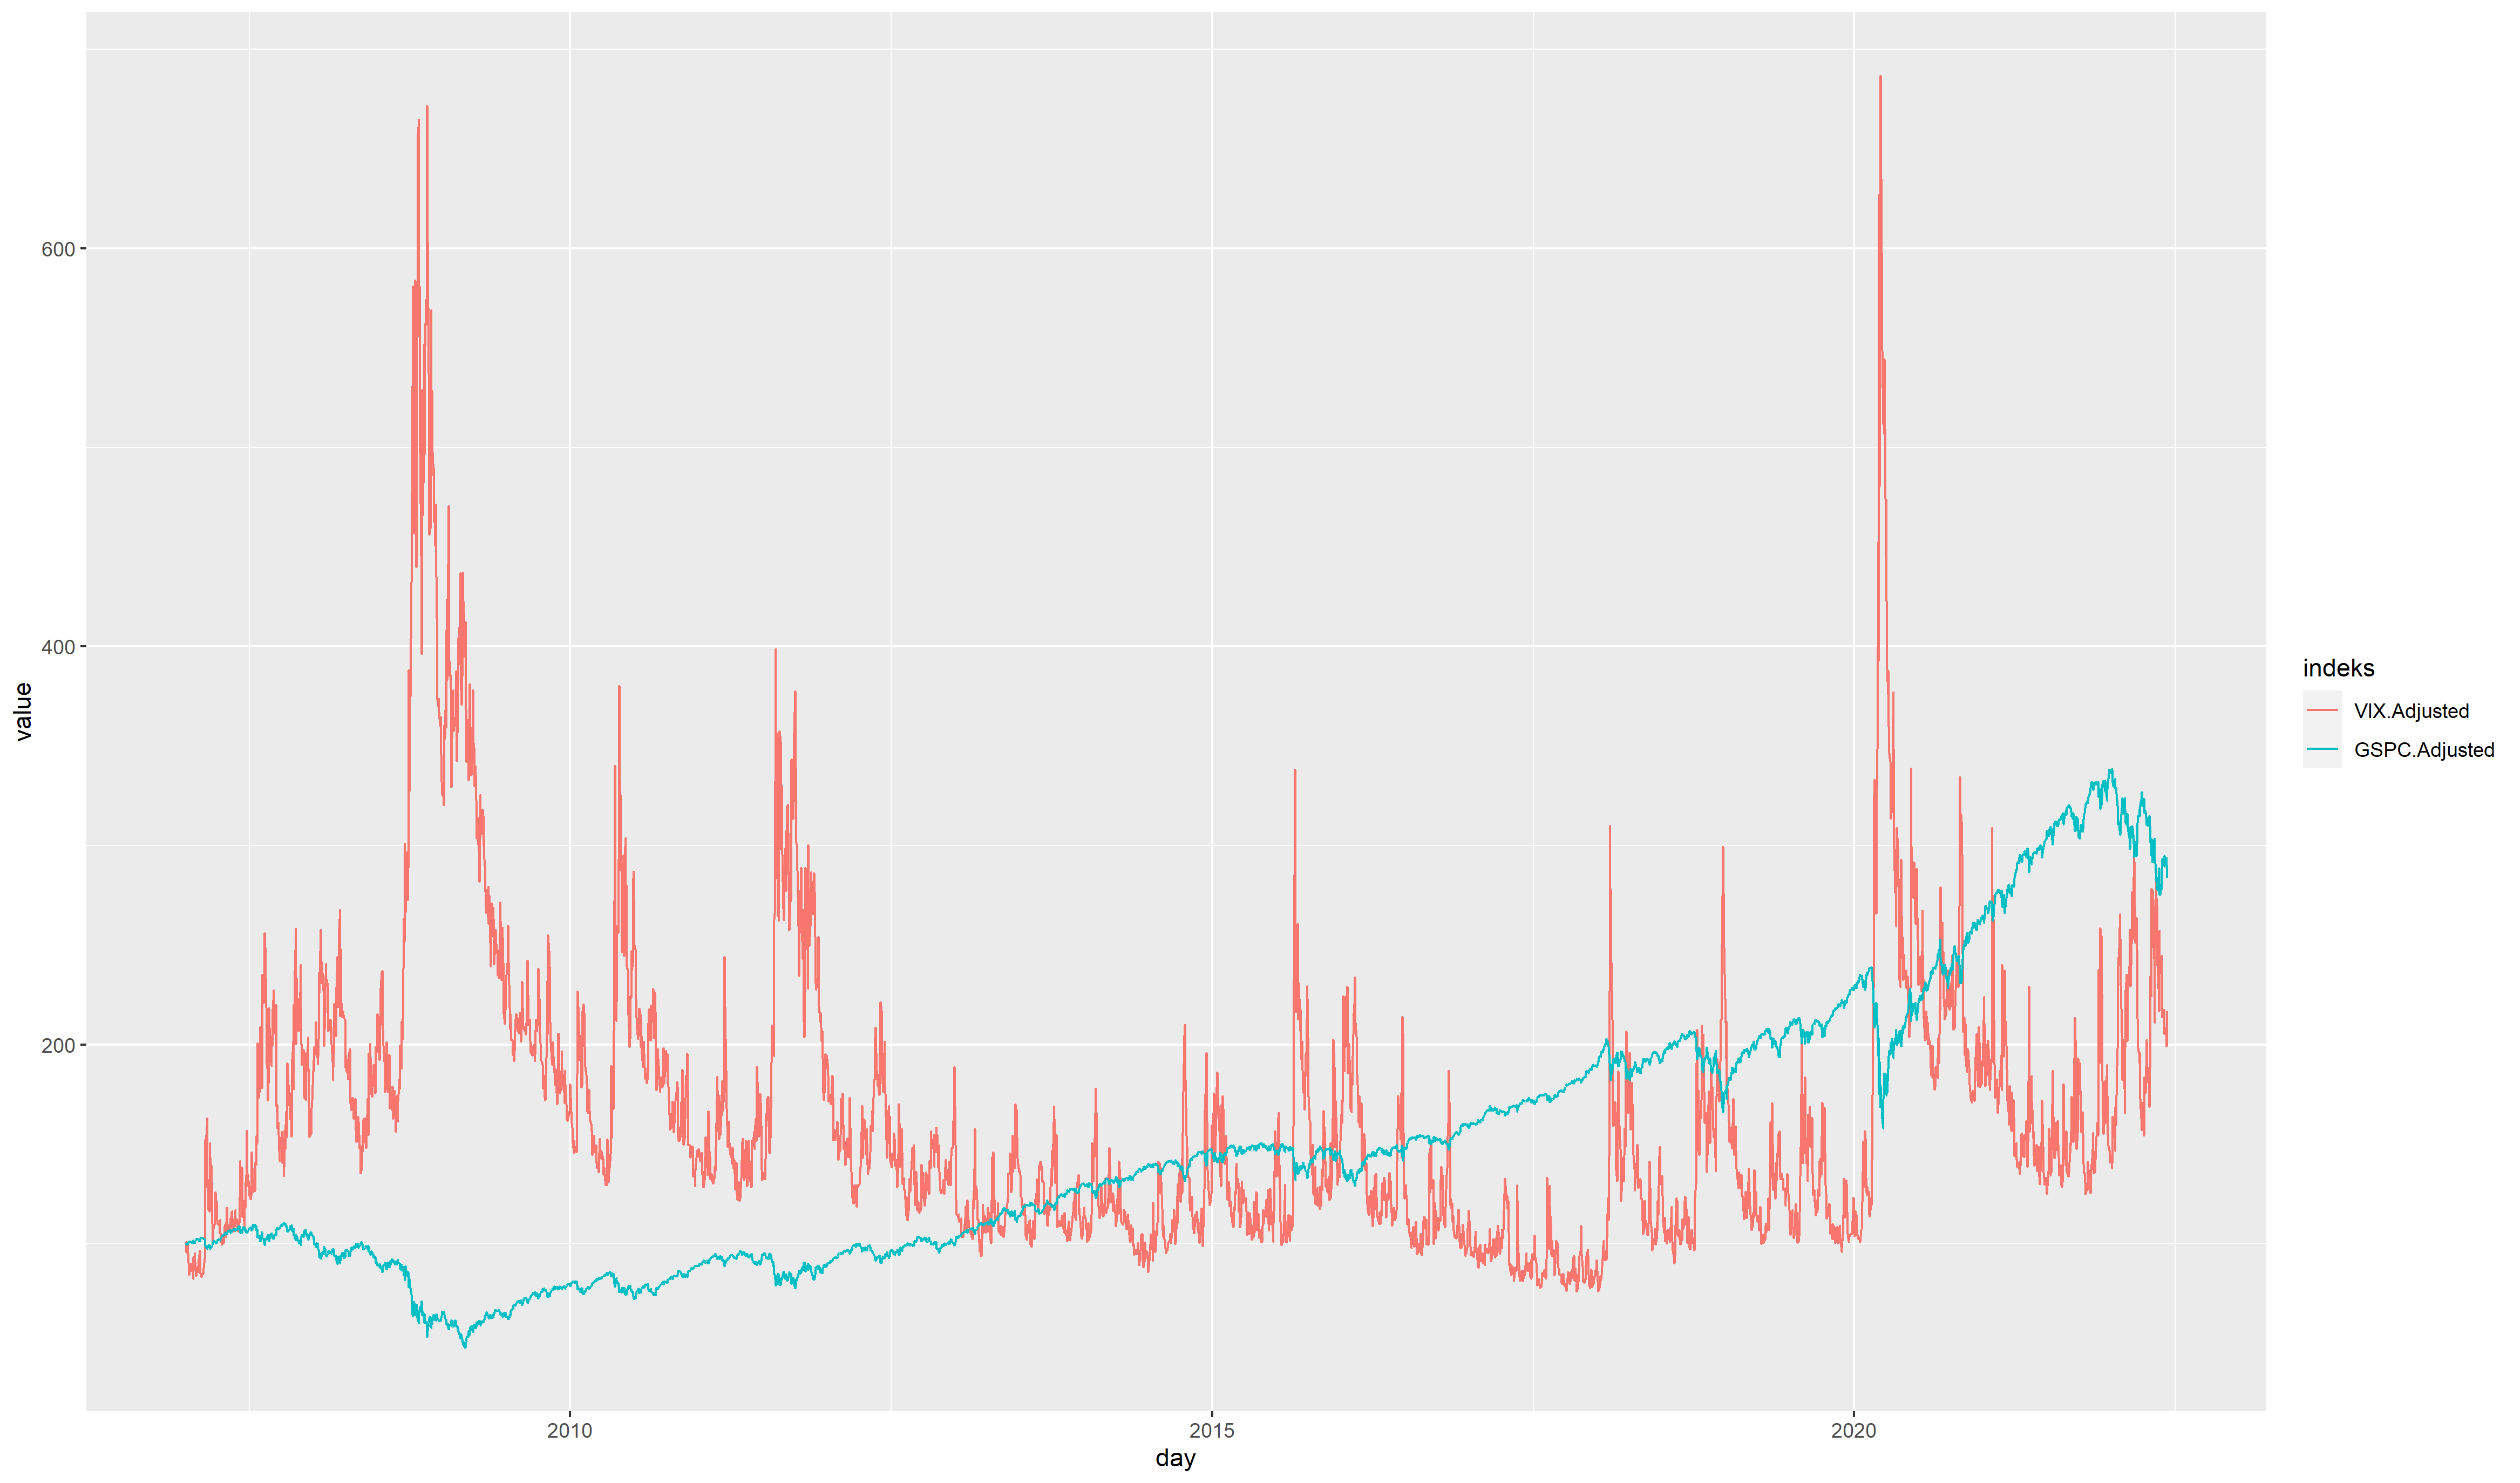
\includegraphics[width=3.5in]{SP500_vs_VIX.png}
    \caption{En graf over VIX og S\&P500, normeret}
    \label{fig:VIXSP500}
\end{figure}
Her ses det at S\&P500 har langt mindre volatilitet når normeret, og vi kan måske ane en tilnærmelsesvist konstant drift. Man kunne derfor tænke sig at sige, at denne er tættere på at kunne simuleres af en geometrisk brownsk bevægelse, da driften er næsten konstant, og volatiliteten ser ud til ved første øjekast kun at afhænge af kursen.

Kigger vi på hvorledes S\&P500 er normal fordelt, kan vi se på figur \ref{fig:QQSP500}, at det lader til at være en ok antagelse.
\begin{figure}
    \centering
    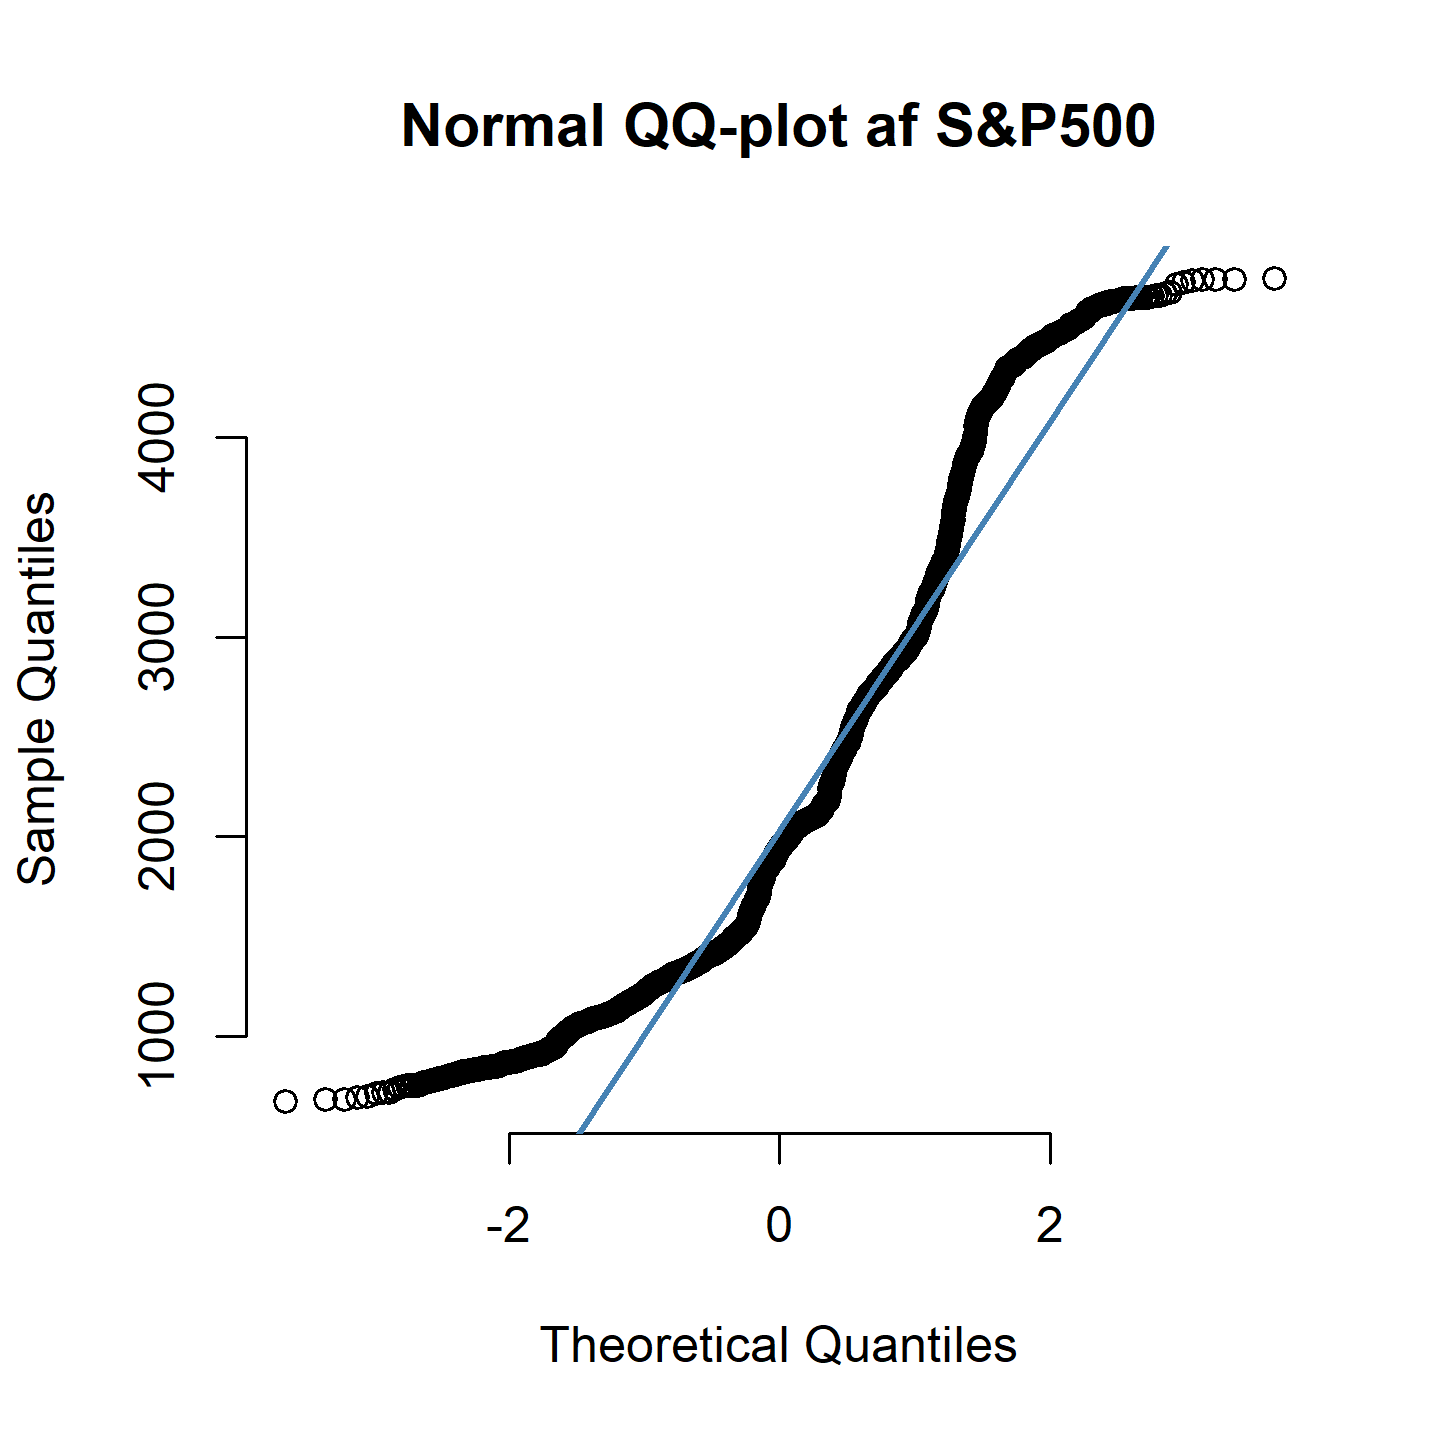
\includegraphics[width=3.5in]{SP500_QQplot.png}
    \caption{Et QQ-plot af S\&P500, normeret}
    \label{fig:QQSP500}
\end{figure}
Ud fra vores teori omkring geometrisk brownsk bevægelse, da ser vi at vores MLE for volatiliteten er
$$\hat{\sigma_{\infty}}=0.28$$
Der ud over kunne man prøve at kigge på MLE for volatiliteten over den seneste financielle måned (i.e. 21 dage) og se, hvordan MLE ændrer sig og på samme tid plotte det eksponentielt vægtede rullende gennemsnit (EWMA) med vægt 0.94. Dette ses på figur \ref{fig:EWMA} og \ref{fig:EWMA_VIX}, nedenfor. 
\begin{figure}
    \centering
    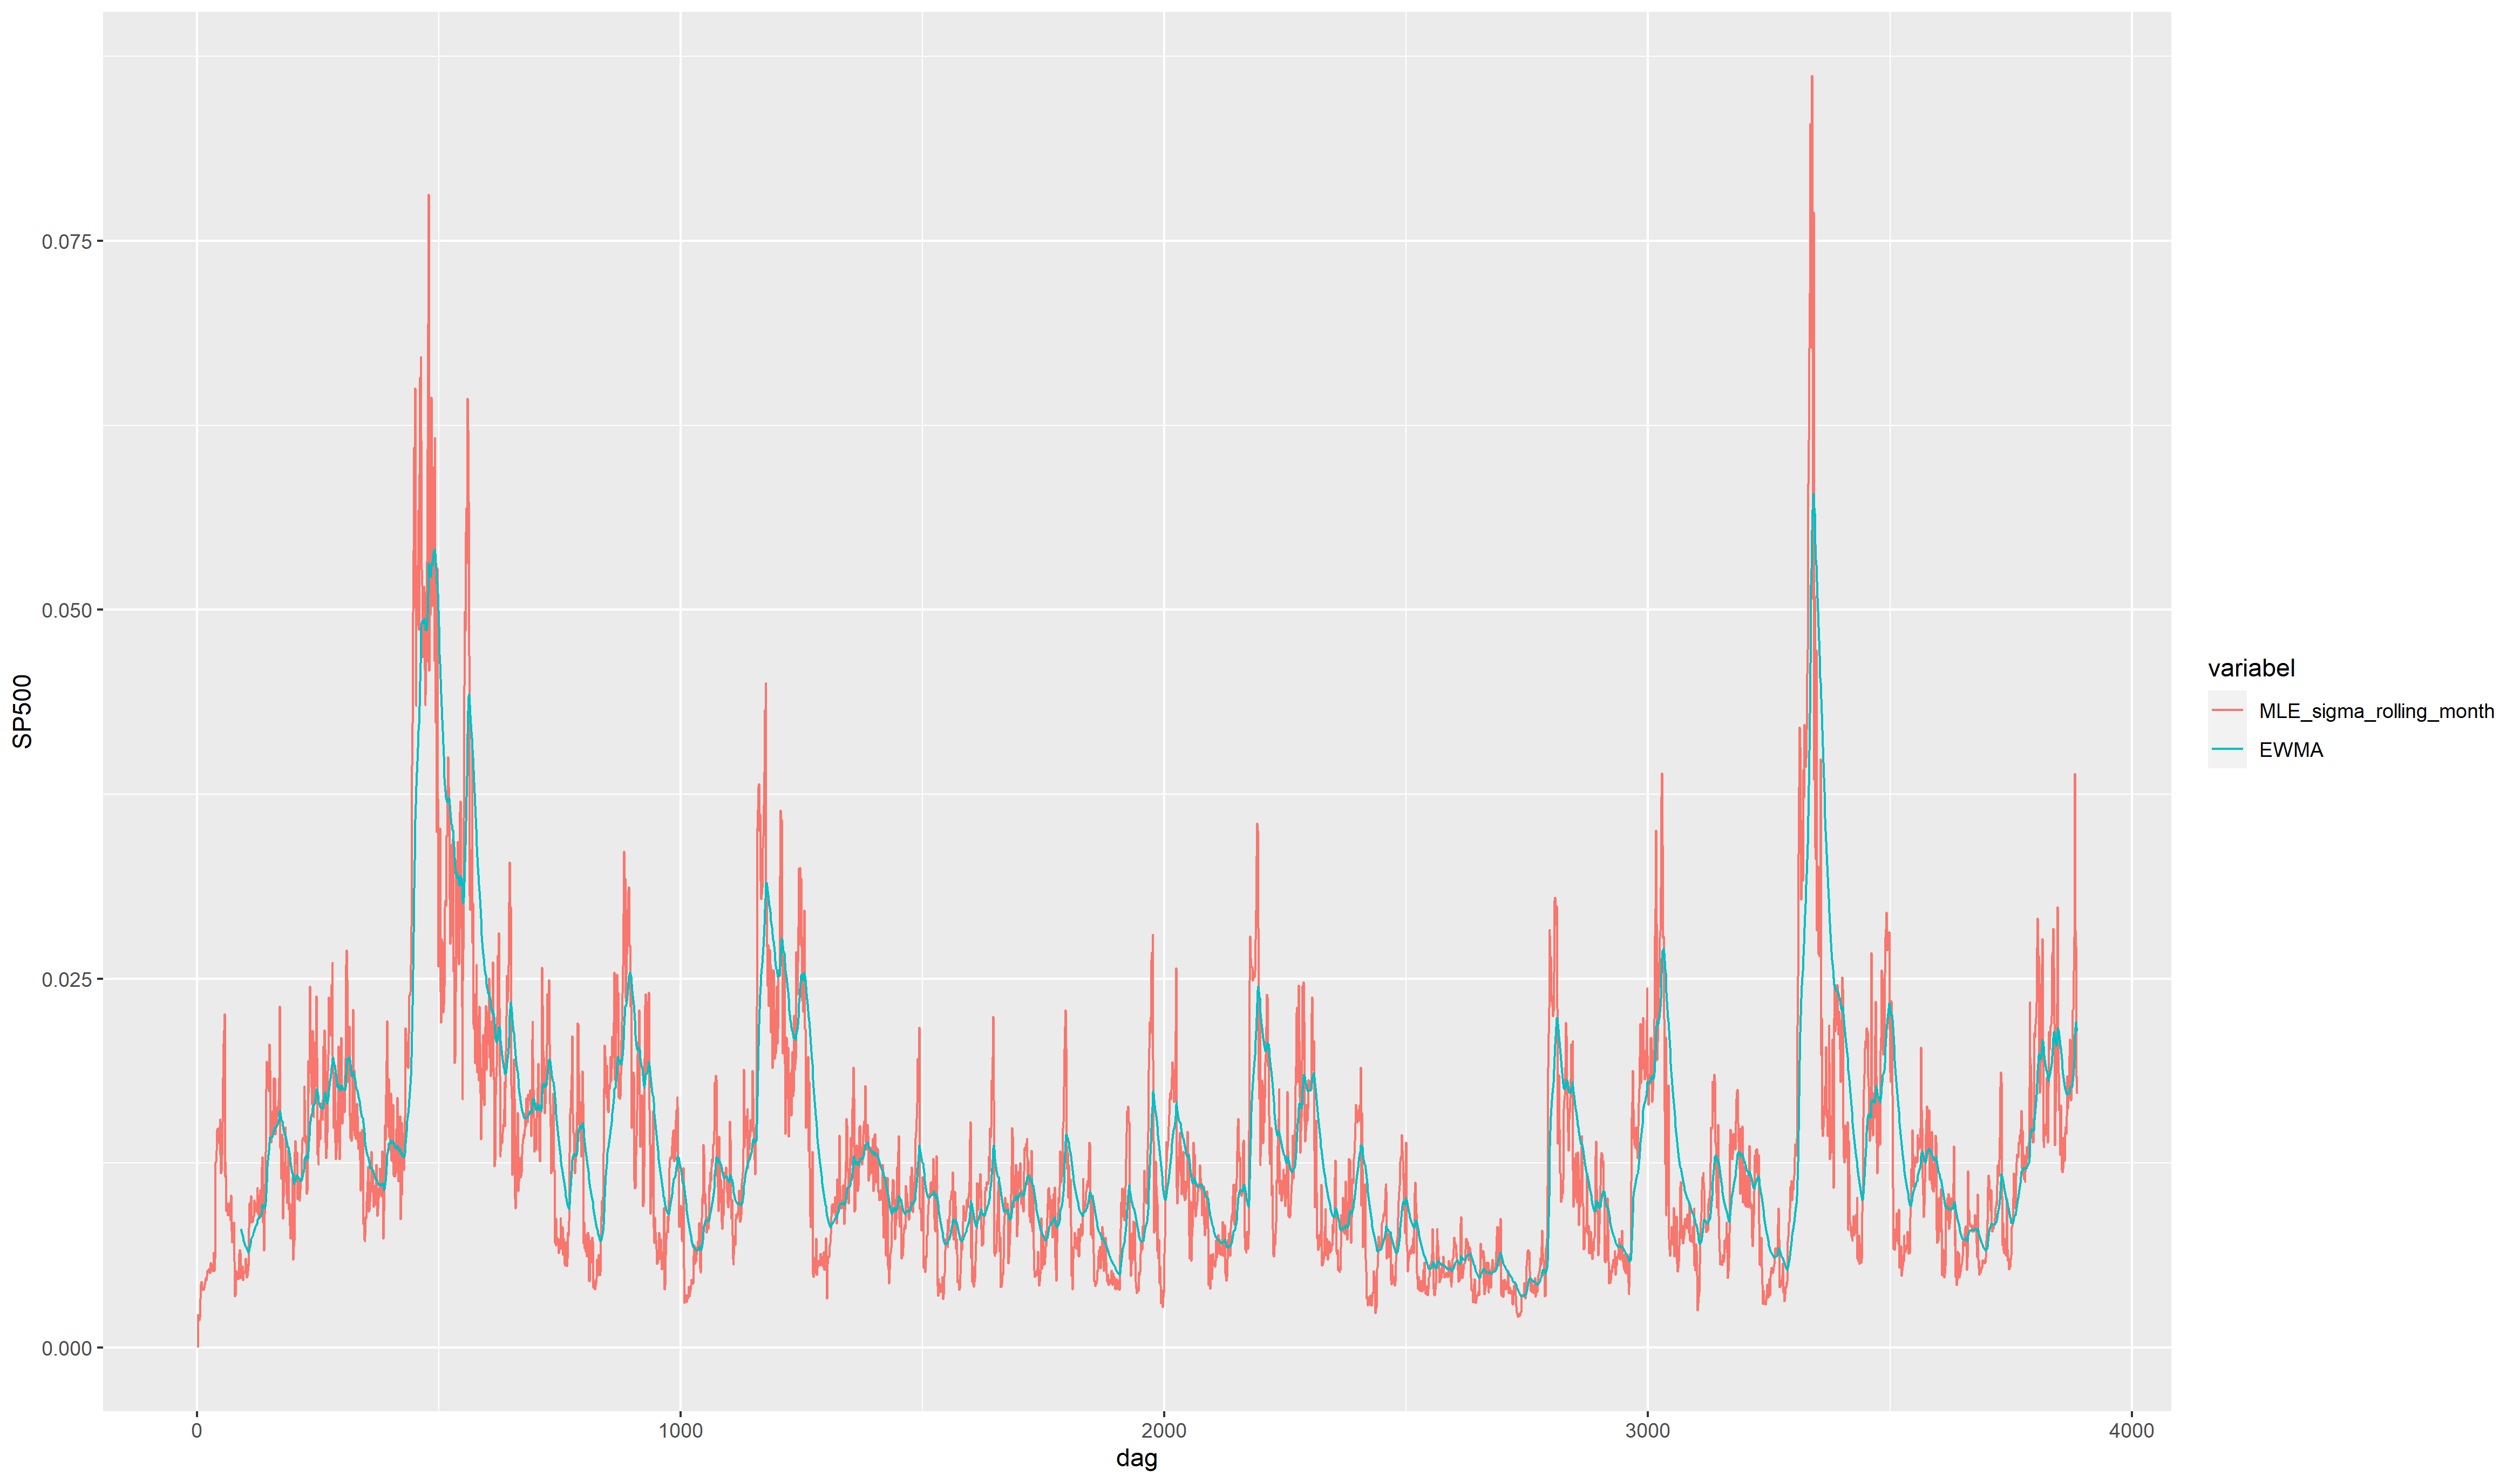
\includegraphics[width=3.5in]{SP500_rolling_volatility.png}
    \caption{Månedlig rullende MLE og EWMA for S\&P500}
    \label{fig:EWMA}
\end{figure}
\begin{figure}
    \centering
    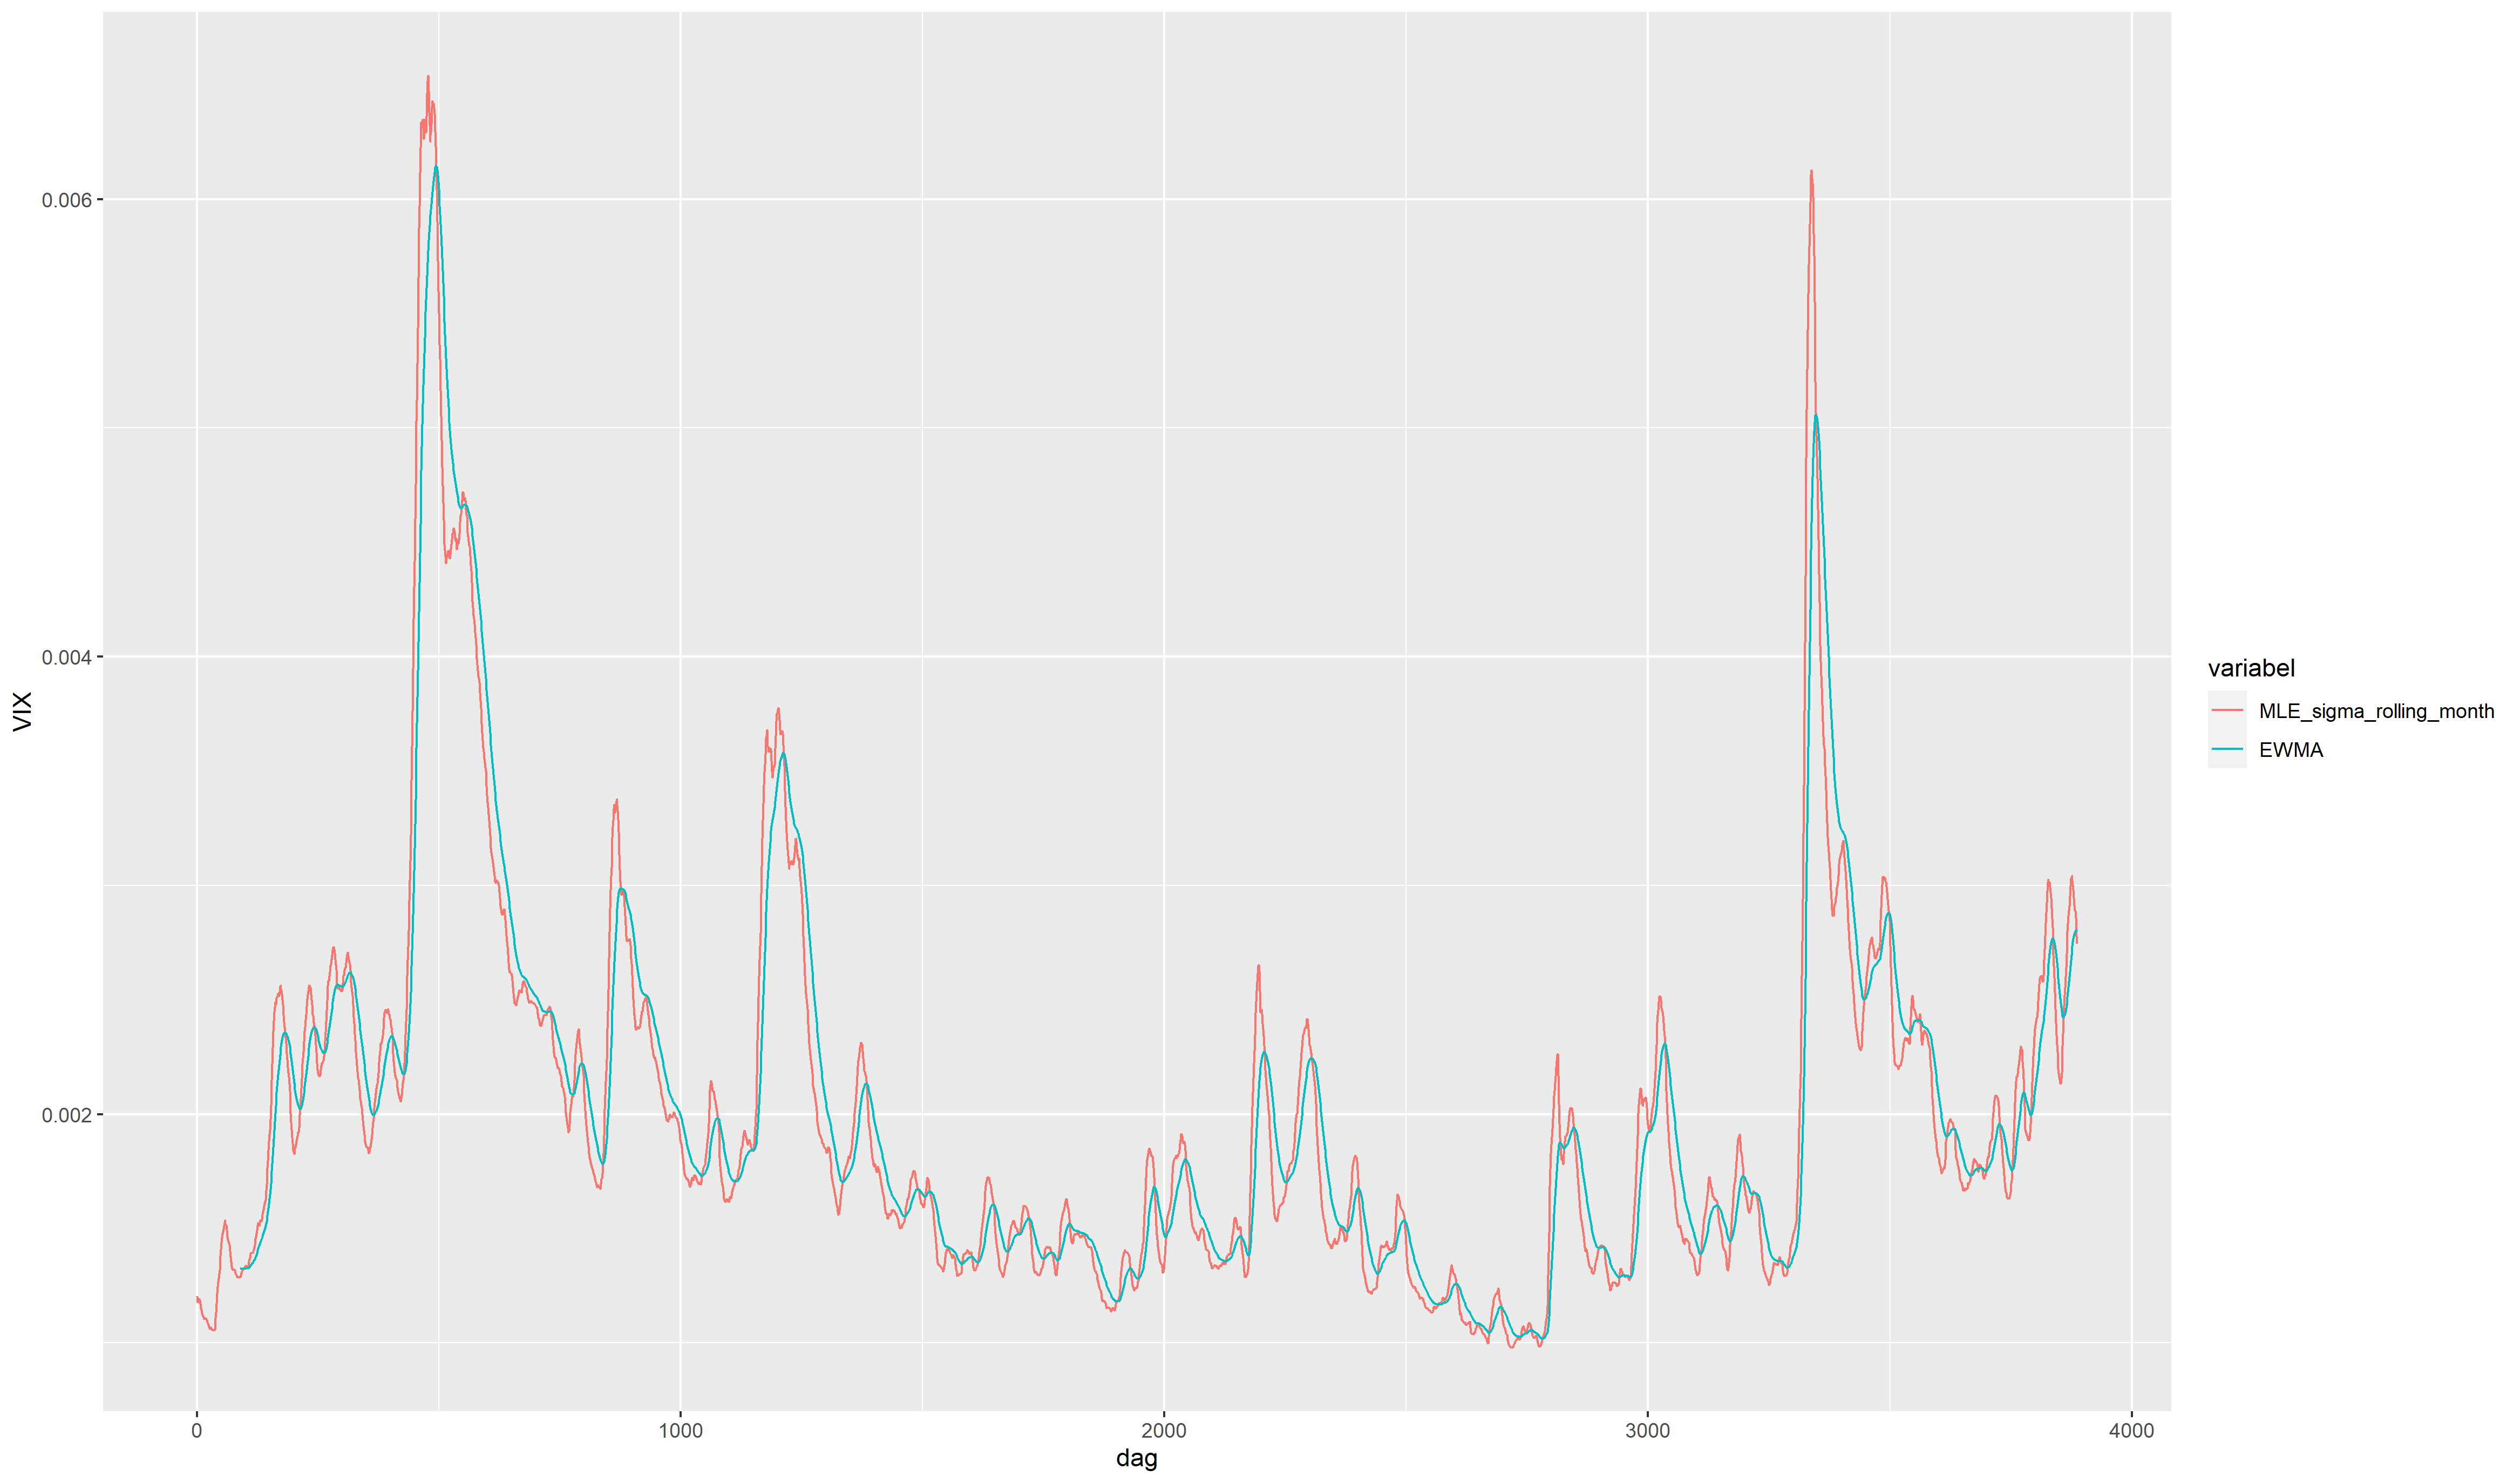
\includegraphics[width=3.5in]{VIX_rolling_volatility.png}
    \caption{Månedlig rullende MLE og EWMA for VIX}
    \label{fig:EWMA_VIX}
\end{figure}

Her indser vi at S\&P500 har et par måder vi kunne estimere dens volatilitet på. F.eks. kunne vi vælge at kigge på VIX istedet for. Der ud over kunne vi kigge på enkelte måneder ad gangen, så vi får glattet vores volatiliteter lidt ud (Dette ville være smart da middelværdier er følsomme overfor outliers). Derudover kunne vi prøve at vægte nyligt hentede observationer højere end gamle ved brug af det eksponentielt vægtede rullende gennemsnit (EWMA)
$$\text{S\&P500 rullende:}\quad\hat{\sigma_{\infty}}=0.0130$$
$$\text{S\&P500 EWMA:}\quad\hat{\sigma_{\infty}}=0.0139$$
$$\text{VIX rullende:}\quad\hat{\sigma_{\infty}}=0.00201$$
$$\text{VIX EWMA:}\quad\hat{\sigma_{\infty}}=0.00203$$
Lad os nu prøve at delta hedge på S\&P500
\begin{figure}
    \centering
    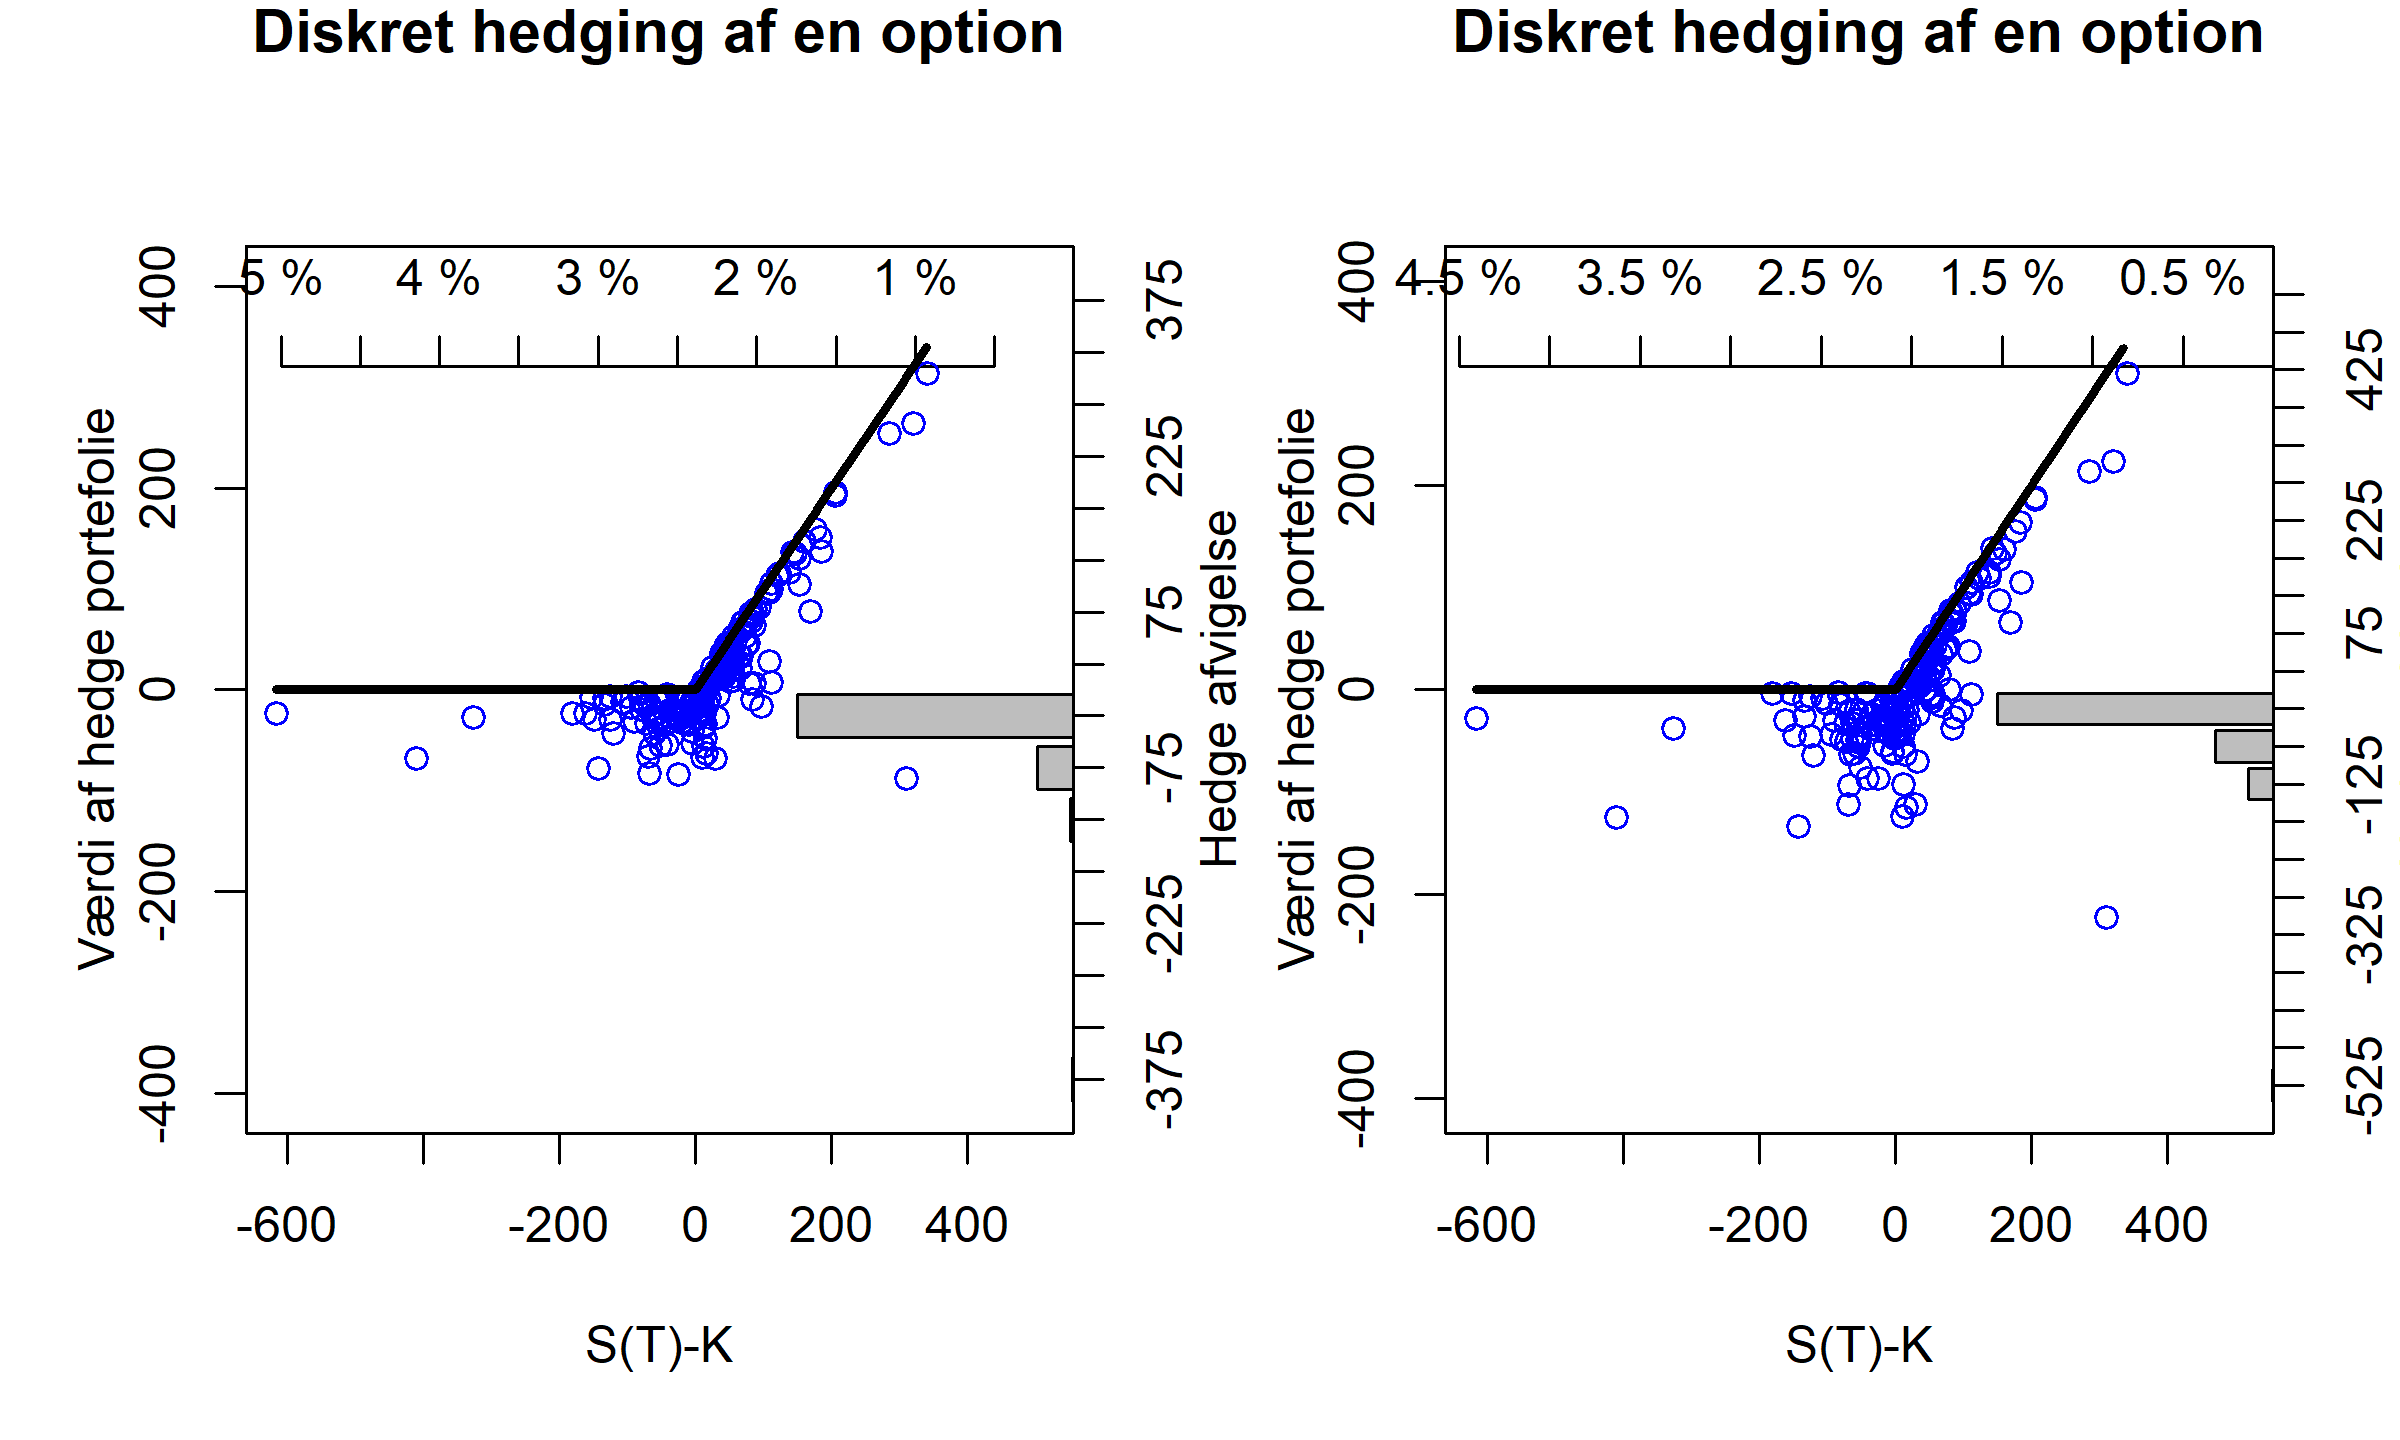
\includegraphics[width=3.5in]{Overleaf/option_call_monthlyGBM_meanVIX100}
    \caption{Venstre: Hver måned udregnes GBM'ens volatilitet, Højre: hver måned udregnes månedens middelværdi af VIK/100}
    \begin{verbatim}
        "-----------------------"                         
                                             "Standard"   "mean(VIX/100)"
        "Average discounted option payoff =    39.43          39.43
        "Average discounted portfolio value =  10.27          1.830
        "Terminal Hedge error mean =           29.16          37.60
        "Terminal Hedge error SD =             29.15          36.02
        "-----------------------"
    \end{verbatim}
    \label{fig:standard}
\end{figure}
\begin{figure}
    \centering
    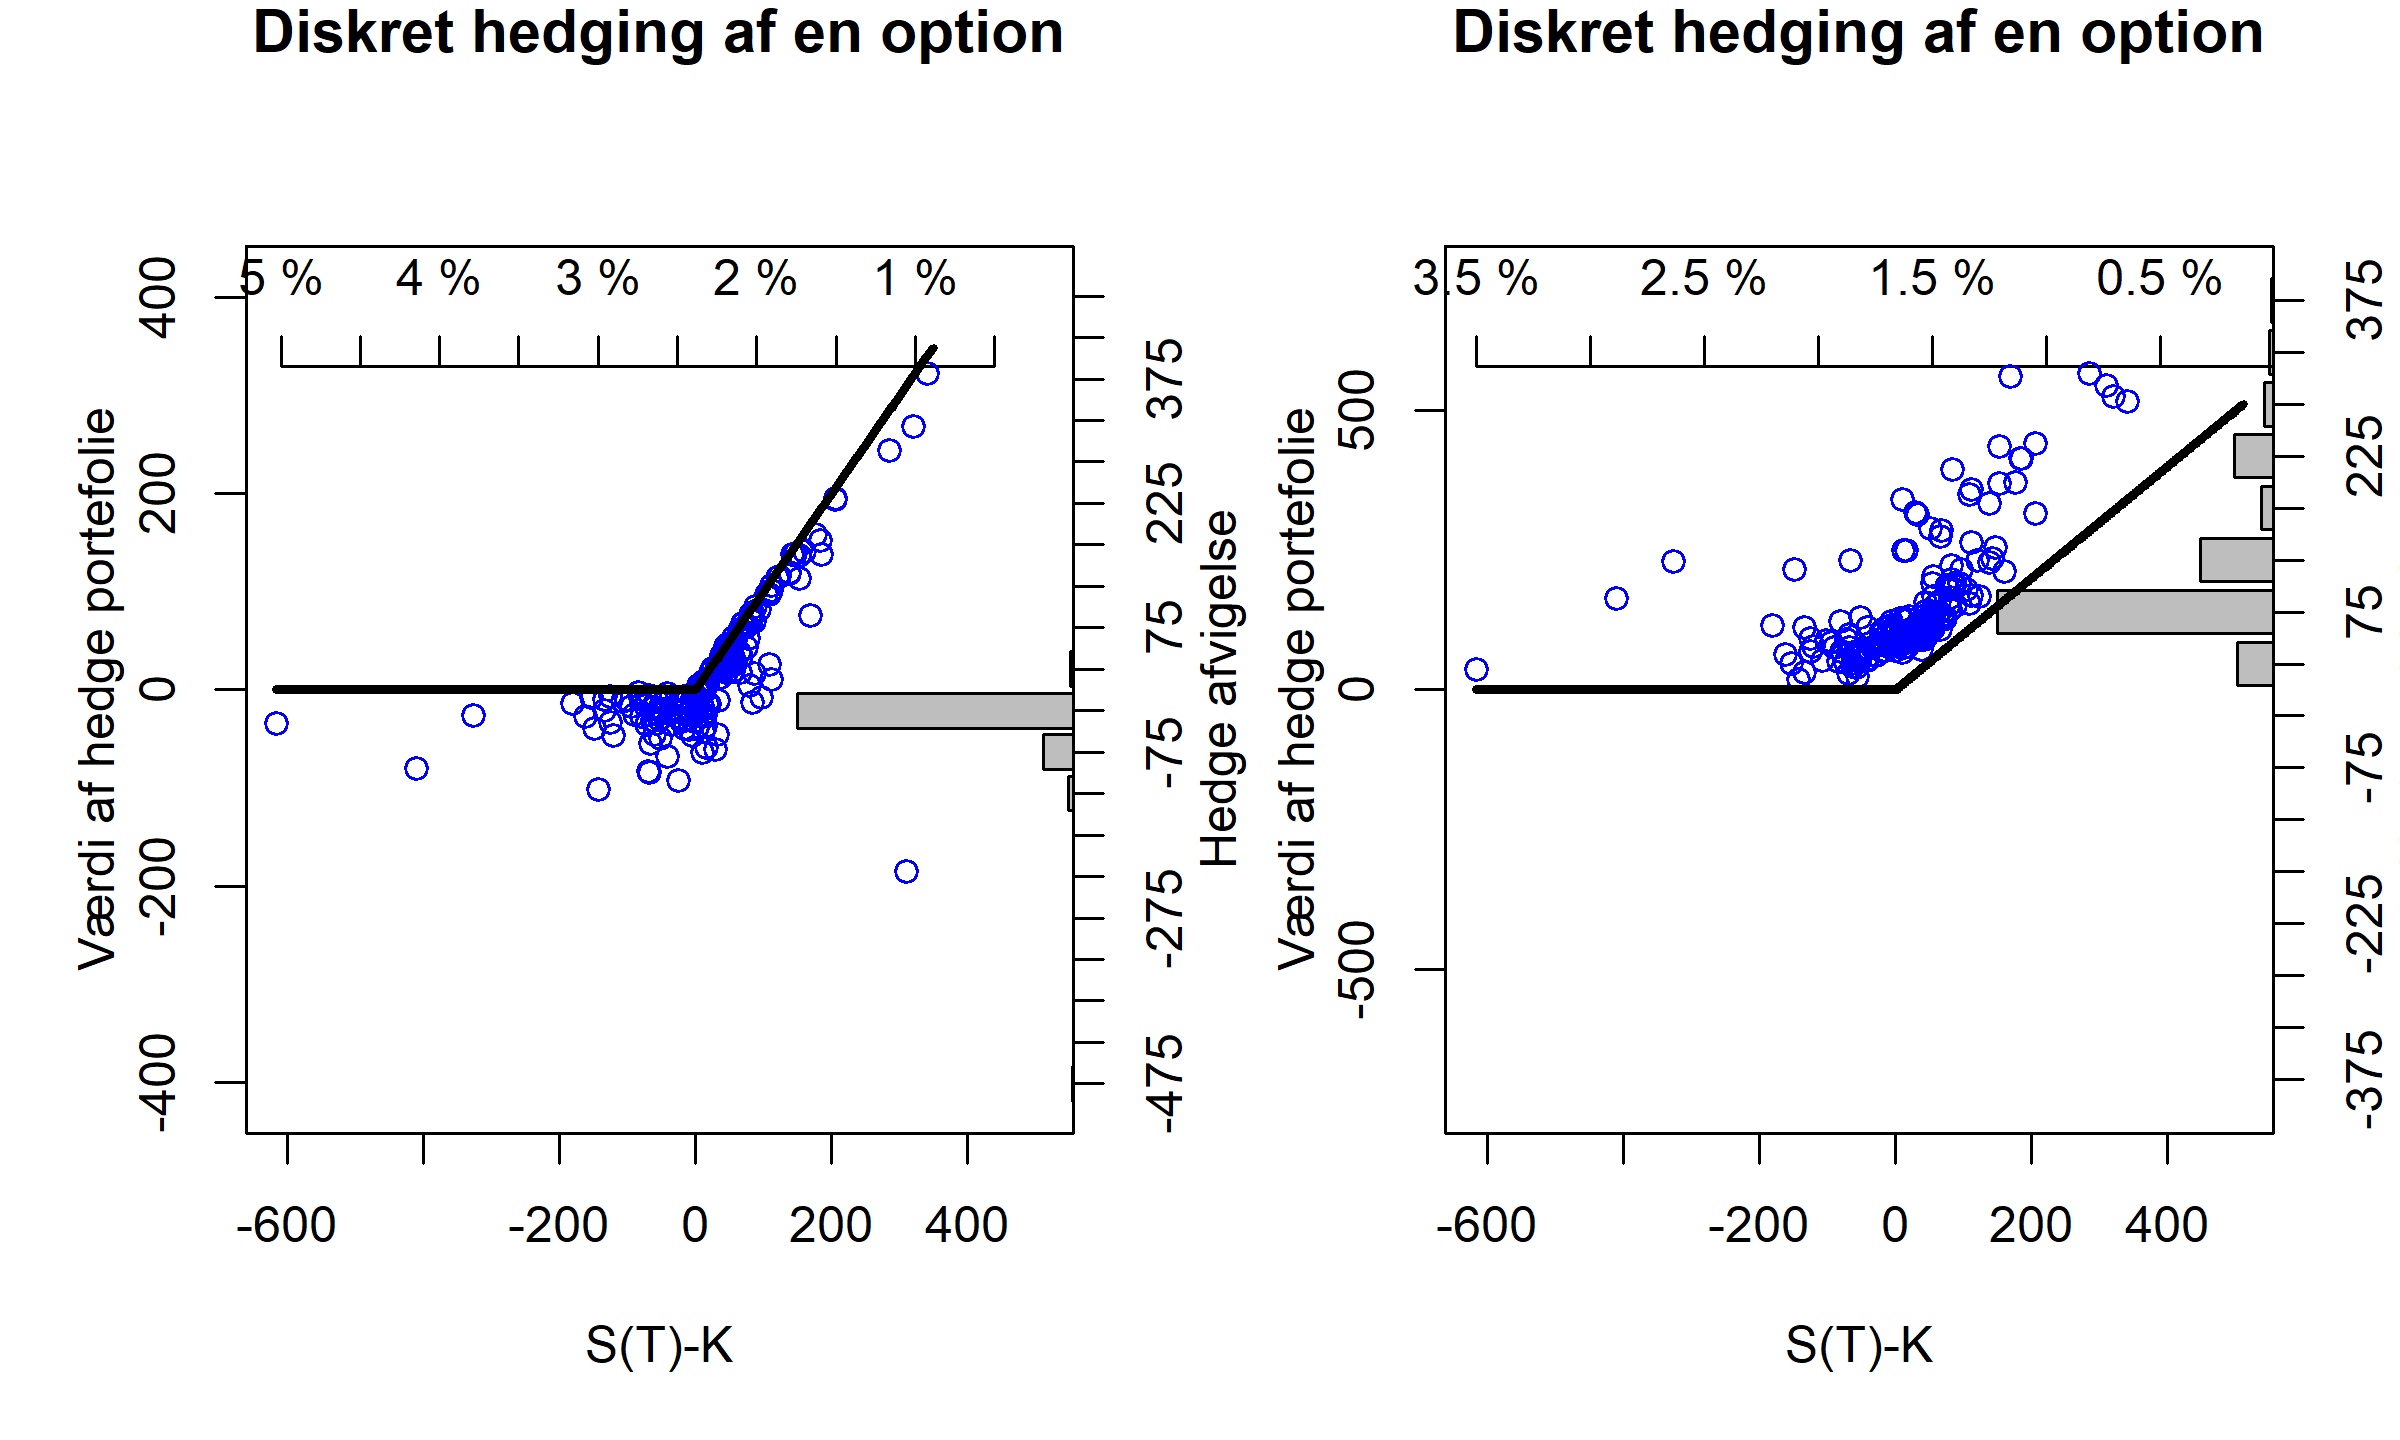
\includegraphics[width=3.5in]{Overleaf/option_call_monthlyGBM_monthlyVIX100EWMA}
    \caption{Venstre: Middel værdi af hver måneds GBM's volatilitet, Højre: middel værdi af alle månedens dage, hvor der hver dag er udregent EWMA 21 dage til bage}
    \begin{verbatim}
        "-----------------------"                         
                                             "Vesntre"       "Højre"
        "Average discounted option payoff =    39.43          39.43
        "Average discounted portfolio value =  11.72          143.9
        "Terminal Hedge error mean =           27.71          104.4
        "Terminal Hedge error SD =             29.80          69.18
        "-----------------------"
    \end{verbatim}
    \label{fig:monthGBM}
\end{figure}


\begin{figure}
    \centering
    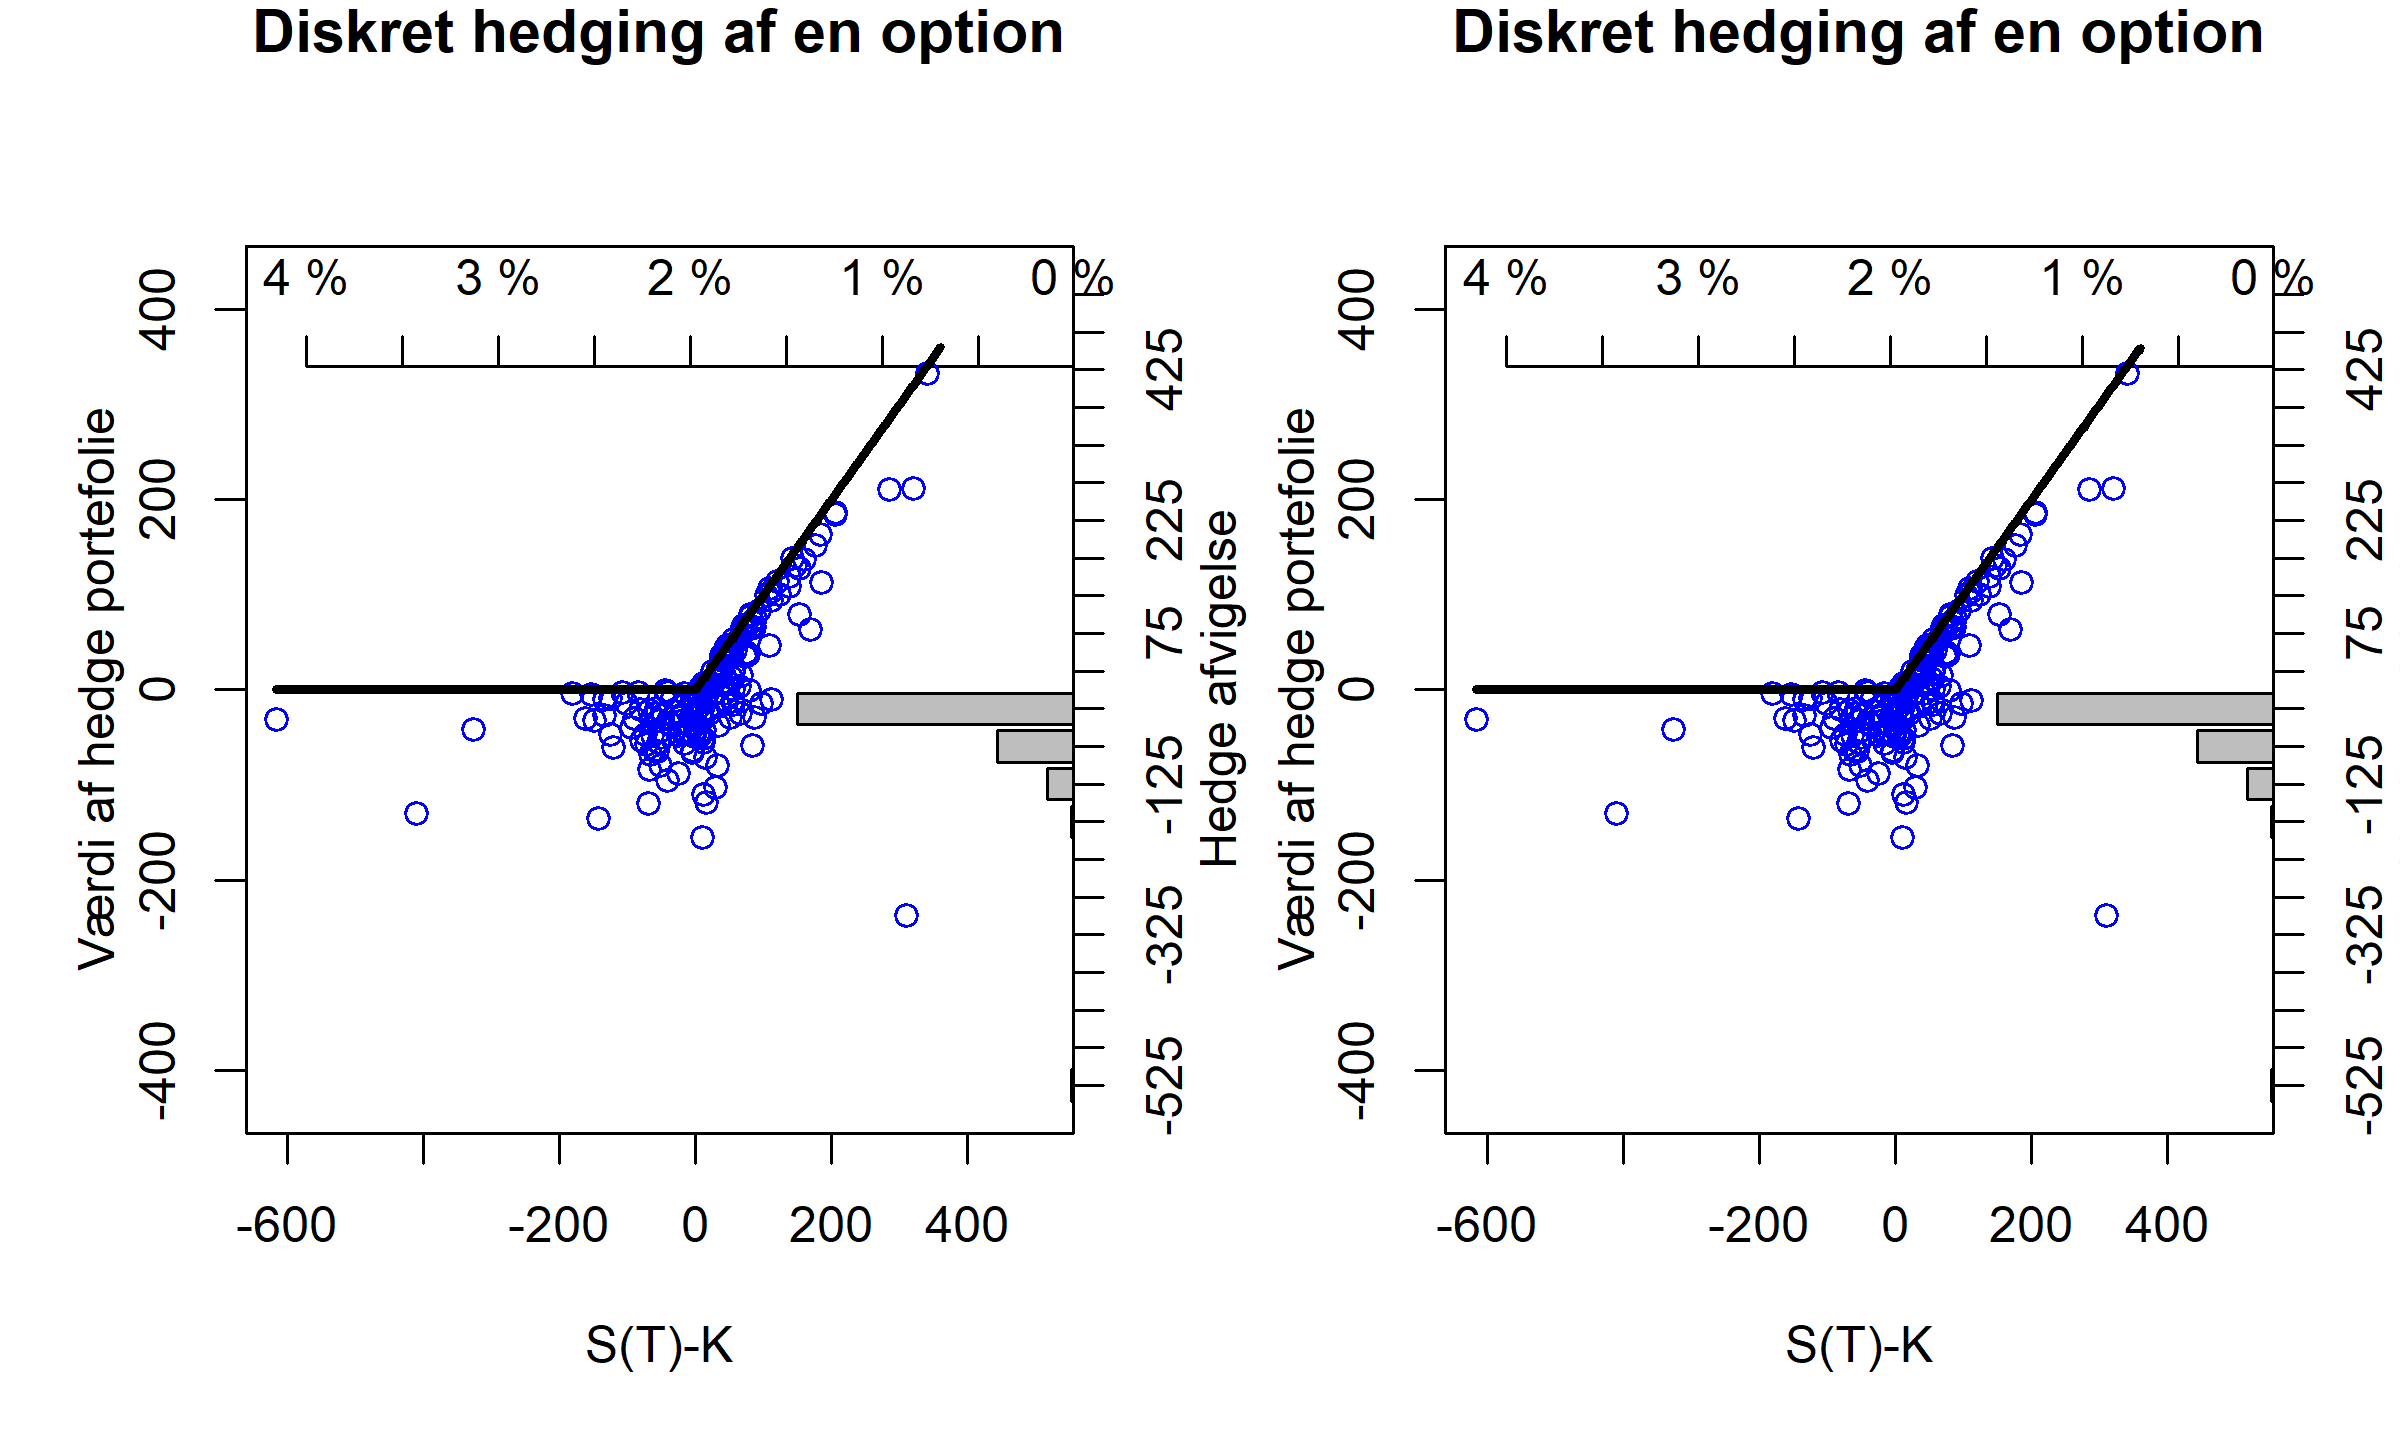
\includegraphics[width=3.5in]{1 product_call_meanrolling_meanEMVA}
    \caption{Venstre: volatiliteten her er et rullende vindu af GBM'ens volatilitet, Højre: EWMA af venstre's udregninger, Begge: til sidst er der taget et gennemsnit for måneden (til venstre er det dermed et gennemsnit af volatiliteter)}
    \begin{verbatim}
        "-----------------------"                         
                                             "Vesntre"       "Højre"
        "Average discounted option payoff =    39.43          39.43
        "Average discounted portfolio value =  1.009          1.011
        "Terminal Hedge error mean =           38.42          38.42
        "Terminal Hedge error SD =             37.26          37.27
        "-----------------------"
    \end{verbatim}
    \label{fig:rullende}
\end{figure}
\begin{figure}
    \centering
    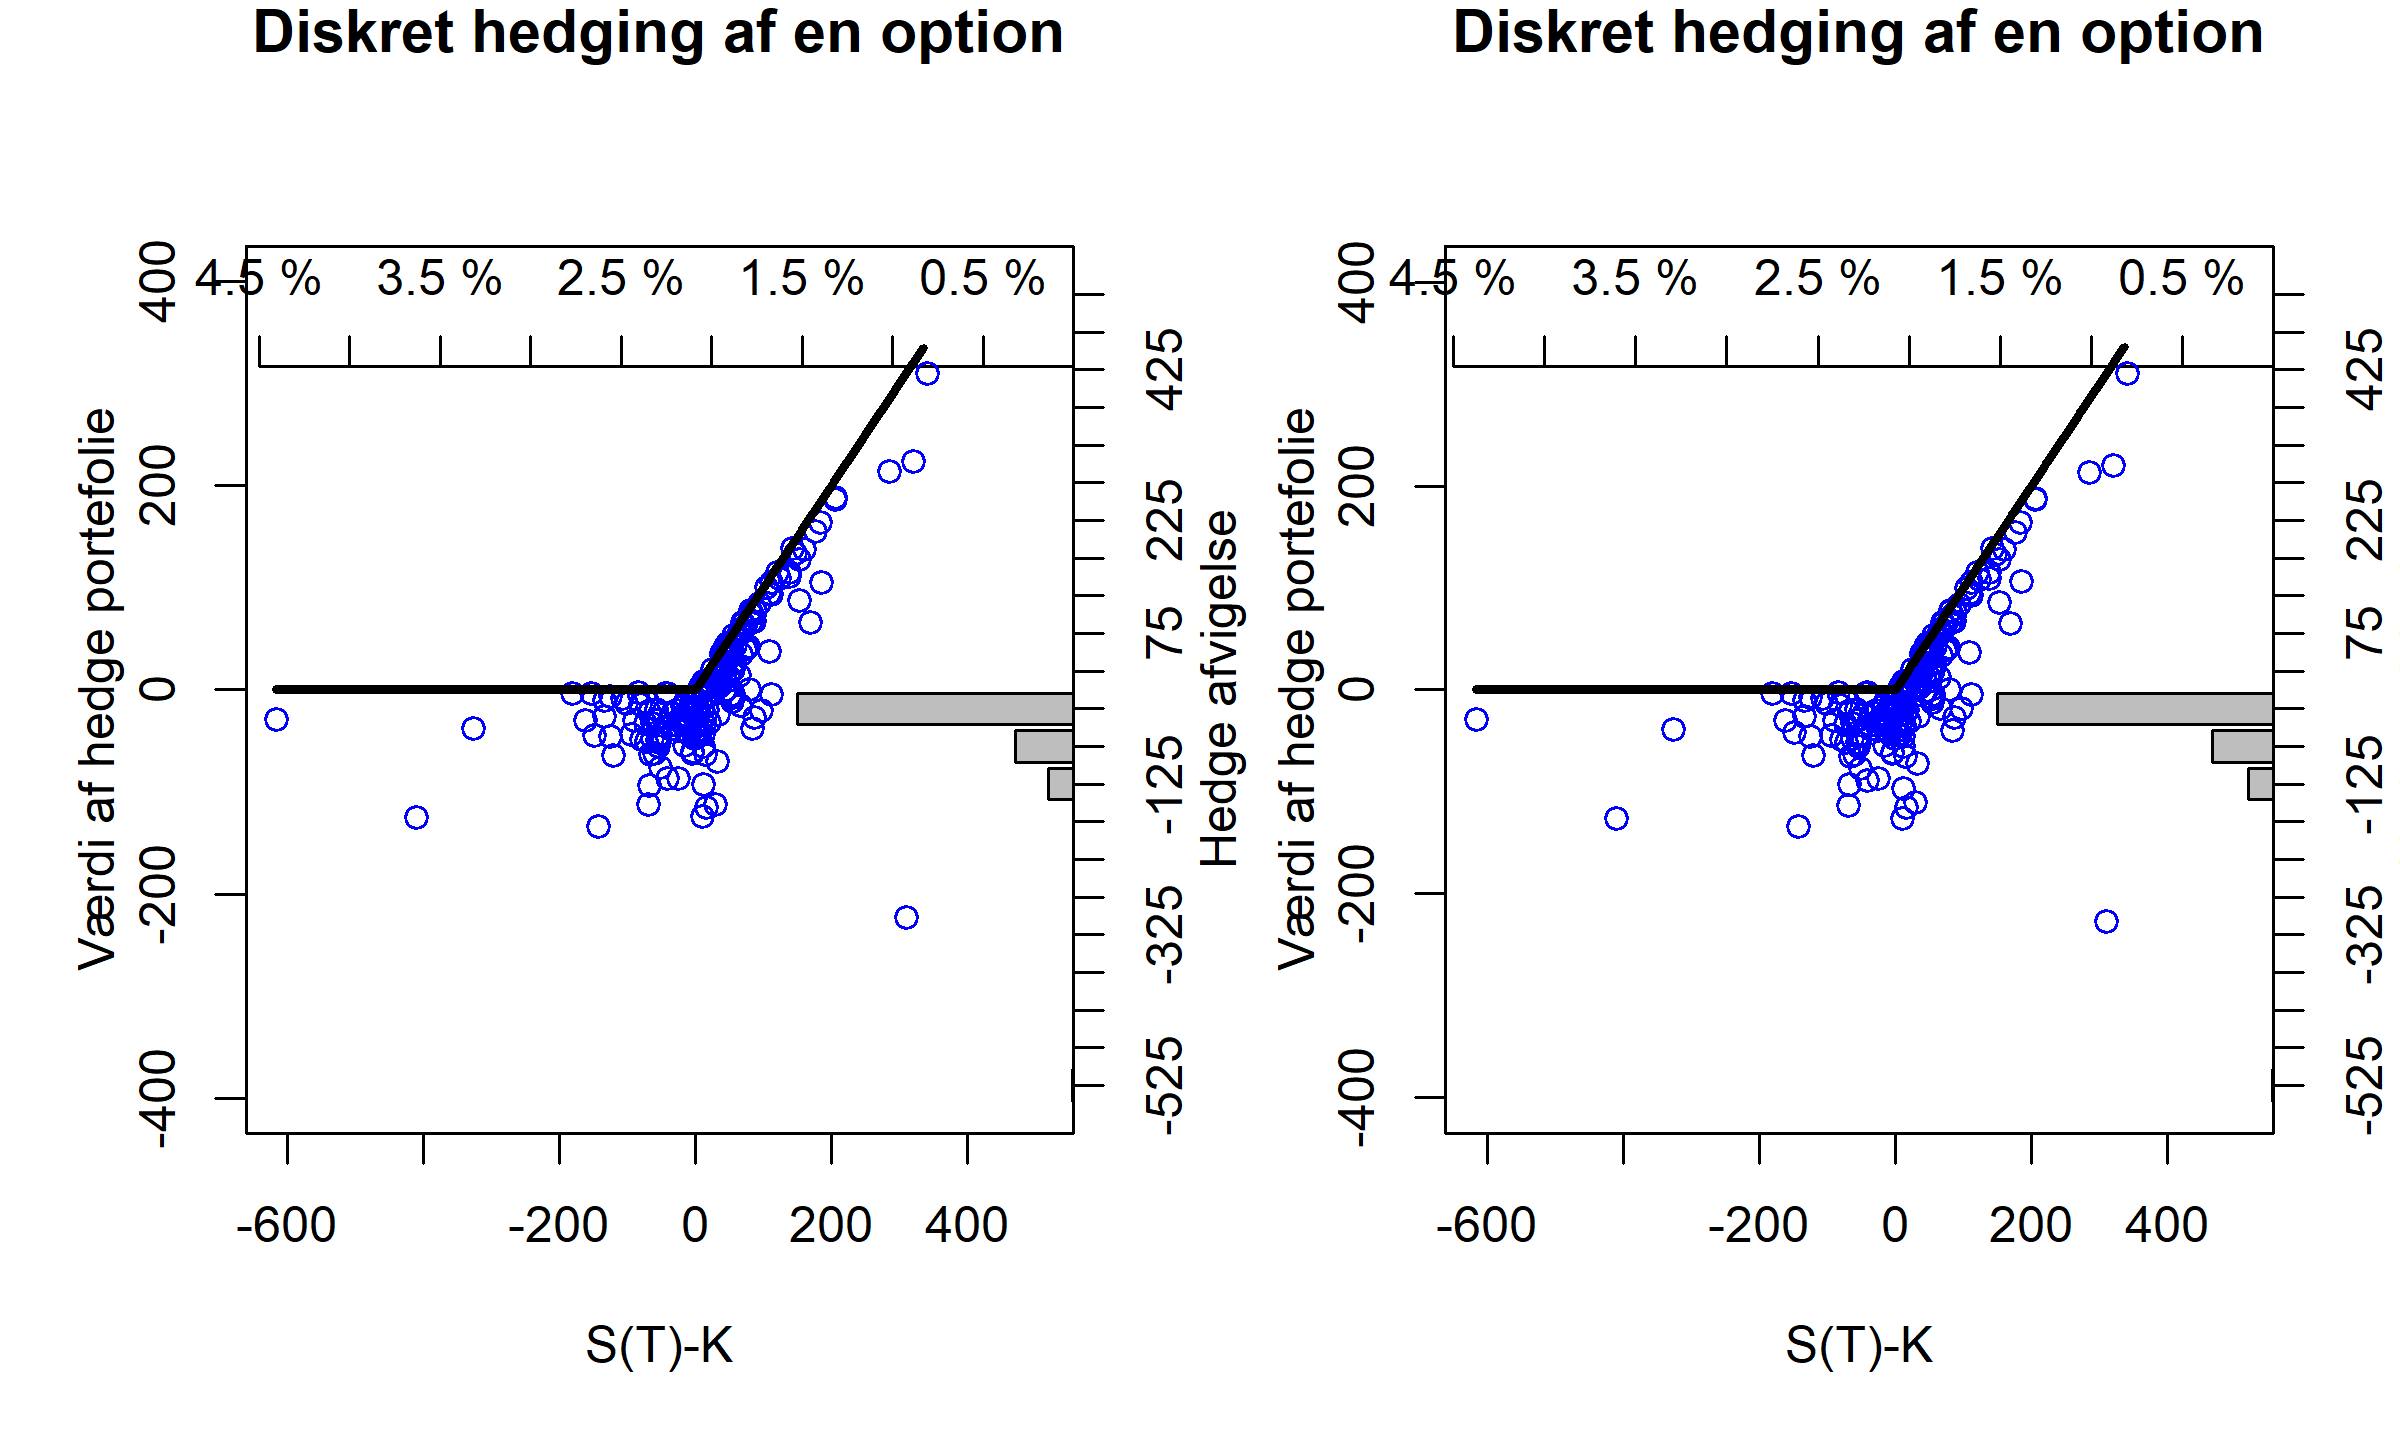
\includegraphics[width=3.5in]{2 product_call_meanrolling_meanEMVA}
    \caption{Venstre: volatiliteten her er et rullende vindu af mean(VIX/100), Højre: EWMA af venstre's udregninger, Begge: til sidst er der taget et gennemsnit for måneden (der er altså tale om en gennemsnit af gennemsnit til venstre)}
    \begin{verbatim}
        "-----------------------"                         
                                             "Vesntre"       "Højre"
        "Average discounted option payoff =    39.43          39.43
        "Average discounted portfolio value =  1.827          1.615
        "Terminal Hedge error mean =           37.60          37.82
        "Terminal Hedge error SD =             36.02          36.27
        "-----------------------"
    \end{verbatim}
    \label{fig:rullendeVIX}
\end{figure}

Vi ser altså at det bedste resultat fremkommer ved, at man tager gennemsnittet af alle månedernes estimerede $\sigma_\text{hedge}$ fra afsnit 3.1, og dermed ikke skifter $\sigma_\text{hedge}$ fra måned til måned som det ses i figur \ref{fig:monthGBM}. Gør man det alligevel, ser vi i figur \ref{fig:standard}, at man opnår relativt gode resultater sammenlignet med den før nævnte.

Både rullende vinduer med middelværdier, og eksponentielt vægtede rullende gennemsnit, lader ikke til at give specielt gode resultater på vores højre figur \ref{fig:monthGBM}, hvor der ses, at den gennemsnitslige fejl er på 104, og som ulig alle de andre ikke har hedge fejl, der ligger i det negative men snare alle er positive. Dette er allarmerende da vi har set fra simulationseksperimentet figur \ref{fig:my_label4} at forkerte $\sigma_\text{hedges}$ burde give negative hedge fejl, når vi kigger på call optioner som vi jo gør her.

Dog er der ingen af vores forsøg i dette afsnit, der indikerer, at vores model faktisk passer (dvs. at vores S\&P500 er en geometrisk brownsk bevægelse). Havde det været det, ville vi have set hedge fejl der ligger trykt omkring 0 som set på venstre figur \ref{fig:my_label4}. Man kunne hurtigt skyde skylden på vores konstante $\sigma$ i modellen, da dette vil give en masse negative fejl som set i højre figur \ref{fig:my_label4}, hvor vi brugte et forkert $\sigma$, ligesom vi også ser her. Dette kan dog ikke forklare vores enorme hedge errors, der det meste af tiden udgør 3/4-del af størrelsen på vores tilbagediskonterede option. Vi må altså konkludere at S\&P500 ikke er en geomtrisk brownsk bevægelse.
\newpage
\section{Konklusion}
Mens vores Black-Scholes model virker præcis som vi vil have den skal i vores simulations eksperiment, hvor vi sørger for, at teoriens antagelser om, at dataen følger en geometrisk brownsk bevægelse ikke er brudt. Da ser vi i praksis, at dette ikke er tilfældet. Et af problemerne kunne være at volatiliteten i virkeligheden nok afhænger af tiden; noget som vores model ikke kan tage højde for på nogen anden måde end at være skaleret med aktie kursen. Det samme kunne siges om driften (omend volatiliteten virker som et stører problem); især når vi ofte taler om bull and bear markets, hvor vi ved at driften har vendt sig.

En model der roder bod på de bekymringer der er rejst her er Heston modellen. En idé til en forbedring af denne afhandling kunne derfor være at bruge den før nævnte model i stedet for Black-Scholes.
\newpage


\phantomsection

\addcontentsline{toc}{section}{Litteratur}
\addcontentsline{toc}{subsection}{Björk}
\addcontentsline{toc}{subsection}{Steffensen}
\bibliographystyle{plain}
\bibliography{references.bib}

\end{document}

